%%%%%%%%%%%%%%%%%%%%%%%%%%%%%%%%%%%%%%%%%%%%%%%%%%%%%%%%%%%%%%%%%%%%%%%%%%%%%%%%
%2345678901234567890123456789012345678901234567890123456789012345678901234567890
%        1         2         3         4         5         6         7         8

\documentclass[letterpaper, 10 pt, conference]{ieeeconf}  % Comment this line out if you need a4paper

%\documentclass[a4paper, 10pt, conference]{ieeeconf}      % Use this line for a4 paper

\IEEEoverridecommandlockouts                              % This command is only needed if 
                                                          % you want to use the \thanks command

\overrideIEEEmargins                                      % Needed to meet printer requirements.

%In case you encounter the following error:
%Error 1010 The PDF file may be corrupt (unable to open PDF file) OR
%Error 1000 An error occurred while parsing a contents stream. Unable to analyze the PDF file.
%This is a known problem with pdfLaTeX conversion filter. The file cannot be opened with acrobat reader
%Please use one of the alternatives below to circumvent this error by uncommenting one or the other
%\pdfobjcompresslevel=0
%\pdfminorversion=4

% See the \addtolength command later in the file to balance the column lengths
% on the last page of the document

% The following packages can be found on http:\\www.ctan.org
%\usepackage{graphics} % for pdf, bitmapped graphics files
%\usepackage{epsfig} % for postscript graphics files
%\usepackage{mathptmx} % assumes new font selection scheme installed
%\usepackage{times} % assumes new font selection scheme installed
%\usepackage{amsmath} % assumes amsmath package installed
%\usepackage{amssymb}  % assumes amsmath package installed

% some very useful LaTeX packages include:

%\usepackage{cite}      % Written by Donald Arseneau
                        % V1.6 and later of IEEEtran pre-defines the format
                        % of the cite.sty package \cite{} output to follow
                        % that of IEEE. Loading the cite package will
                        % result in citation numbers being automatically
                        % sorted and properly "ranged". i.e.,
                        % [1], [9], [2], [7], [5], [6]
                        % (without using cite.sty)
                        % will become:
                        % [1], [2], [5]--[7], [9] (using cite.sty)
                        % cite.sty's \cite will automatically add leading
                        % space, if needed. Use cite.sty's noadjust option
                        % (cite.sty V3.8 and later) if you want to turn this
                        % off. cite.sty is already installed on most LaTeX
                        % systems. The latest version can be obtained at:
                        % http://www.ctan.org/tex-archive/macros/latex/contrib/supported/cite/

\usepackage[dvips]{graphicx}  % Written by David Carlisle and Sebastian Rahtz
                        % Required if you want graphics, photos, etc.
                        % graphicx.sty is already installed on most LaTeX
                        % systems. The latest version and documentation can
                        % be obtained at:
                        % http://www.ctan.org/tex-archive/macros/latex/required/graphics/
                        % Another good source of documentation is "Using
                        % Imported Graphics in LaTeX2e" by Keith Reckdahl
                        % which can be found as esplatex.ps and epslatex.pdf
                        % at: http://www.ctan.org/tex-archive/info/

%\usepackage{amsmath}   % From the American Mathematical Society
                        % A popular package that provides many helpful commands
                        % for dealing with mathematics. Note that the AMSmath
                        % package sets \interdisplaylinepenalty to 10000 thus
                        % preventing page breaks from occurring within multiline
                        % equations. Use:
\usepackage{multirow}
\usepackage[left=0.71in,top=0.94in,right=0.71in,bottom=1.18in]{geometry}
\setlength{\columnsep}{0.24in}
% correct bad hyphenation here
%\hyphenation{op-tical net-works semi-conduc-tor IEEEtran}

   \usepackage{amsmath}
   \usepackage{amsbsy}
   \usepackage{setspace}
   \usepackage{fancyhdr}
   \usepackage{color}
   \usepackage{commath}   
   \usepackage{array}
   \usepackage{psfrag}
   \usepackage{epsfig}


% ------------------------------
%  ALIASES
% ------------------------------
%
%   \newcommand{\eqref}[1]{(\ref{#1})}

\newcommand{\beq}{\begin{equation}}
\newcommand{\eeq}{\end{equation}}
\newcommand{\bea}{\begin{eqnarray}}
\newcommand{\eea}{\end{eqnarray}}
\usepackage{amssymb}
\usepackage{graphicx}

\newtheorem{lemma}{Lemma}
\newtheorem{theorem}{Theorem}
\newtheorem{definition}{Definition}
\newtheorem{property}{Property}
\newtheorem{assumption}{Assumption}
\newtheorem{remark}{Remark}

   \newcommand{\clearemptydoublepage}{\newpage{\pagestyle{empty}\cleardoublepage}}
   \newcommand{\later}{\vspace{5cm}}
%
   \newcommand{\bdm}{\small\begin{displaymath}}
   \newcommand{\edm}{\end{displaymath}\normalsize}
%   \newcommand{\beq}{\small\begin{equation}}
%   \newcommand{\eeq}{\end{equation}\normalsize}
%   \newcommand{\beqa}{\small\begin{eqnarray}}
%   \newcommand{\eeqa}{\end{eqnarray}\normalsize}
   \newcommand{\nn}{\nonumber}
   \newcommand{\bit}{\begin{itemize}}
   \newcommand{\eit}{\end{itemize}}
   \newcommand{\ds}{\bigcirc}
%
   \renewcommand{\b}[1]{\mbox{\boldmath$#1$}}
\newcommand{\Ad}{\text{Ad}}

   \newcommand{\eqreff}[1]{(\ref{#1})}
   \newcommand{\grad}{${}^{\circ}$\hspace{0.1cm}}
   \newcommand{\gradm}{{}^{\circ}}
   \def\partfrac#1#2{\frac{\partial{#1}}{\partial{#2}}}
   \def\deltfrac#1#2{\frac{\Delta{#1}}{\Delta{#2}}}
   \def\VecO#1{\underline{#1}}
   \def\TenO#1{\underline{\underline{#1}}}
   \def\MatO#1{\boldsymbol {\mathrm{#1}}}
   \def\VecMatO#1{\underline{\mbox{\bf {#1}}}}
   \def\Vec#1#2{\underline{#1}\:\!{}^{#2}}
   \def\Ten#1#2{\underline{\underline{#1}}\:\!{}^{#2}}
   \def\Mat#1#2{\boldsymbol{\mathrm{#1}}\:\!{}^{#2}}
   \def\VecMat#1#2{\underline{\mbox{\bf{#1}}}\:\!{}^{#2}}
   \def\Sum#1#2{\sum_{#1}^{#2}}
   \def\Prod#1#2{\prod_{#1}^{#2}}
   \def\Diff#1#2#3{{}^{{}^{{}^{{}^{\scriptstyle #1}}}} \! \frac{d#2}{d#3}}
   \def\const{\mbox{const.}}
   \def\cs{\mbox{c}}
   \def\sn{\mbox{s}}
   \def\diag{\mbox{diag}}
%
%   \definecolor{hellgrau}{gray}{0.96}
   \def\graybox#1{\colorbox{hellgrau}{\parbox[r]{\textwidth}{#1}} }
   \def\linebox#1{\fbox{\parbox[r]{\textwidth}{#1}} }
%
   \newenvironment{intro}{\begin{quote}\small\it}{\end{quote}}
%


\newcommand{\FontFigXXS}{.5}
\newcommand{\FontFigXS}{.6}
\newcommand{\FontFigSS}{.7}
\newcommand{\FontFigS}{.8}
\newcommand{\FontFigM}{1}
\newcommand{\FontFigB}{1.3}
\newcommand{\FontFigBBB}{20}
\newcommand{\FontFigBB}{15}

% color red
\newcommand{\rev}[1]{{\color{black}{{#1}}}}
\newcommand{\rek}[1]{{\color{black}{{#1}}}}


\title{
Tracking Control for the Grasping of a \rev{Non-Cooperative} Tumbling Satellite with a Free-Floating Robot
}

\author{Roberto Lampariello, Hrishik Mishra, Nassir Oumer, Phillip Schmidt, Marco De Stefano, Alin Albu-Sch\"affer% <-this % stops a space
\thanks{All authors are from the Institute of Robotics and Mechatronics (DLR), 82234 We\ss ling, 
Germany, email: \textit{firstname.lastname@dlr.de}}%
}



\begin{document}



\maketitle
\thispagestyle{empty}
\pagestyle{empty}


%%%%%%%%%%%%%%%%%%%%%%%%%%%%%%%%%%%%%%%%%%%%%%%%%%%%%%%%%%%%%%%%%%%%%%%%%%%%%%%%
\begin{abstract}
In this paper a novel method is presented for grasping a \rev{partially cooperative} tumbling satellite with a free-floating robot. A reference trajectory, provided by an offline motion planner and adapted online to account for modelling uncertainties, is tracked with a visual servo for the approach phase and with a joint-space controller for the rigidization phase which follows the grasp. An Extended Kalman filter ensures a Lipschitz continuity of the noisy pose estimates of a visual tracker, which makes the control method robust for executing the grasping task. The visual servo is in cascade with an impedance controller to achieve tracking while being compliant. The method is successfully validated on the OOS-SIM facility, which allows simulating gravity-free multibody dynamics with the hardware-in-the-loop simulation method. 
\end{abstract}

%\begin{IEEEkeywords}
%Space Robotics, Optimization and Optimal Control, Visual Servoing,  Visual Tracking.
%\end{IEEEkeywords}

%%%%%%%%%%%%%%%%%%%%%%%%%%%%%%%%%%%%%%%%%%%%%%%%%%%%%%%%%%%%%%%%%%%%%%%%%%%%%%%%
\section{Introduction}
% 1,25 pp, including abstract and figure 1
%
Among the possible applications of robotic systems in an orbital scenario, this paper focusses on those which may operate in On-Orbit Servicing and in Active Debris Removal missions~\cite{932685}\cite{Shoemaker2003}\cite{dlr63555}\cite{telaar2017gnc}. To tackle the related control challenges we present here an autonomy-based approach, in which the robot is commanded through a precomputed reference trajectory, corrected by a tracking controller, to account for intrinsic planning and execution errors. We focus on the task of grasping a defective, tumbling target satellite (from here on, the Target) by means of a free-floating robot, consisting of a non-actuated chaser satellite (from here on, the Chaser) carrying a kinematically redundant robot manipulator. These are shown in Fig.~\ref{fig:facility}.

The task of grasping a target satellite with a space robot was already performed in \cite{932685} and \cite{Shoemaker2003}, however only for the case of a cooperative Target. When the Target cannot be attitude controlled and does not present \rev{dedicated} visual or structural features to aid its grasping, then it is generally termed non-cooperative. \rev{We consider here the case in which the Target presents a circular rail where it can be grasped, and assume that sufficient information is provided to allow generating a simplified geometric model of it for visual tracking purposes. Also in} this case, the accomplishment of the robotic grasping task in autonomous mode presents some substantial challenges. The robot motion is dictated by that of the Target, which is generally unknown. The robot motion also has to be correctly synchronized with that of the Target, in order to meet and grasp some preselected grasping point on it, while satisfying motion constraints, such as workspace limits, kinematic and dynamic singularities, collision avoidance, as well as sensor-driven constraints, such as camera field-of-view boundaries and pixel velocity limits. Furthermore, due to the given free-floating dynamics in play, the effect of an impact during the contact phase can be very detrimental for accomplishing the task, since it can quickly bring the Target out of the range of the robot.

The grasping task of interest has been addressed extensively in the literature, first in the context of feedback control and then also in that of optimal control (see Section~\ref{sec:related_work}). While in the former the aim is to solve a regulation control problem, often taking advantage of the free-floating dynamics and redundancy of the Chaser, in the latter an open-loop approach is preferred, based on the idea of computing a feasible and optimal trajectory in real-time. Due to the highly constrained task, explained above, the use of a feasible trajectory is recognized to be of great importance.
\begin{figure}[t!]
\psfrag{I1}[cc][cc][\FontFigBBB]{{\color{white}$\{\mathcal{I}\}$}}
\psfrag{t}[cc][cc][\FontFigBBB]{{\color{black}$\{\mathcal{T}\}$}}
\psfrag{g}[cc][cc][\FontFigBBB]{{\color{black}$\{\mathcal{G}\}$}}
\psfrag{e}[cc][cc][\FontFigBBB]{{\color{black}$\{\mathcal{E}\}$}}
\psfrag{b}[cc][cc][\FontFigBBB]{{\color{black}$\{\mathcal{B}\}$}}
\psfrag{q}[cc][cc][\FontFigBB]{{\color{black}$q$}}
\psfrag{r}[cc][cc][\FontFigBB]{{\color{black}$r$}}
\psfrag{g_pose}[cc][cc][\FontFigBB]{{\color{black}$\begin{bmatrix}\eta_t,~ \rho_t \end{bmatrix}$}}
\psfrag{camera}[cc][cc][\FontFigBB]{{\color{black}$\begin{bmatrix}\mu,~ r_c \end{bmatrix}$}}
\psfrag{c_pose}[cc][cc][\FontFigBB]{{\color{black}$\begin{bmatrix}\eta_c,~ \rho_c \end{bmatrix}$}}
\psfrag{t_pose}[cc][cc][\FontFigBB]{{\color{black}$\begin{bmatrix}q,~ r \end{bmatrix}$}}
\centering\includegraphics[angle=0,width=0.47\textwidth]{./figures/motiv1}
\caption{OOS-SIM experimental facility used to reproduce the gravity-free dynamics of the Chaser (left), carrying a Light-Weight Robot, and the Target (right). A camera is mounted on the gripper of the kinematically redundant manipulator, to allow visual servoing. The reference frames of the Chaser $\mathcal{B}$, the robot end-effector $\mathcal{\epsilon}$, the Target $\mathcal{T}$ and the predefined grasping point $\mathcal{G}$ are also shown.}
\label{fig:facility}
%\vspace{-10pt}
\end{figure}

A gap in the methodology described above, which we want to close here, is that of having both the optimal control and the feedback control elements working together. A feedback controller alone does not provide any guarantee of convergence, given the presence of the constraints, which give rise to local minima. Furthermore, the grasping task has a limited time window for its execution and local control methods generally do not ensure finite time convergence. At the same time, an open-loop approach is not robust to modelling errors (e.g., dynamic model) and to contingencies, such as an impact. 

\rev{We therefore present here a tracking controller for executing the grasping task of interest which: firstly, takes as input a reference trajectory from a database, generated off-line with a motion planner in simulation and feasible with respect to all relevant constraints; secondly, superimposes sensor-based corrections to the reference input, to account for the discrepancy between the simulated and the real world. 

To this end, the overall tracking control task is composed of the following two sequential phases. The first phase of the task, the approach phase, is executed by a novel interconnected system which is a cascade of visual servo and an impedance controller. The visual servo appears as an outer-loop velocity command which brings the robot end-effector onto the grasping point on the tumbling Target. It is widely recognized that the robustness of a visual servo is significantly improved against modelling errors when performing tracking rather than regulation~\cite{siciliano2016springer}. The use of impedance control is intended to minimize the detrimental effect of an impact between the robot manipulator and the Target. In the rigidization phase which follows the grasping task, the Target is stabilized with respect to the Chaser using the reference trajectory which in turn exploits the manipulator controller's dissipation to assure that the final configuration for the whole system is reached with a decaying velocity. Furthermore, in this phase, the intrinsic modelling uncertainty in the reference trajectory is handled with an on-line adaptation of the reference trajectory. An additional novelty in the controller is the use of robust estimates of pose and velocity which are obtained from an Extended Kalman Filter (EKF) for feedback and feed-forward respectively. The filter is fed with the noisy, outlier-affected, low-frequency pose estimates of a model-based visual tracking algorithm and produces filtered signals for the tracking controller. It is worth pointing out that the success of the aforesaid controller requires a judicious interplay between the different elements involved: the motion planner, the visual servo (including the EKF and the visual tracking) and the free-floating robot impedance controller. 

In addition to defining the control laws for the aforementioned controller, experimental validations on DLR's OOS-SIM robotic facility, shown in Fig.~\ref{fig:facility}, are also presented. This facility allows reproducing realistic orbital gravity-free dynamics in three-dimensions through hardware-in-the-loop simulation. From an infrastructure perspective, a novel momentum-based approach was also developed for the facility in order to simulate the post-grasping tumbling motion of the compound system which was necessary to validate the concepts presented in this paper.}

The paper is then structured as follows. In the rest of this Section, we present a relevant bibliography and a more detailed problem statement. In Section~\ref{sec:methods} we provide details of the applied methods, while in Section~\ref{sec:results} we present the experimental results and their analysis. Finally, in Section~\ref{sec:disc} we provide a discussion and conclude with remarks outlining the scope of future work. 

The mathematical notation is such that scalar constants are written in plain text, scalar variables in italics, vectors, vector arrays and matrices are always bold, coordinates of vector quantities are expressed with the left upper superscript. The right upper superscript $i\:j$ defined the direction of a vector from $i$ to $j$. \rek{A homogeneous transformation matrix (pose) is denoted as $\mathbf{H} \equiv \mathbf{H}(R(q),r)$, where $q \in \mathbb{R}^4$ and $r \in \mathbb{R}^3$ are the quaternion orientation and the position respectively. A quaternion is written as $\theta = \begin{bmatrix}\theta_v^T& \theta_0\end{bmatrix}$ where $\theta_v \in \mathbb{R}^3$ is the vector part. A pose $\mathbf{H}$ is driven by a twist $\dot{\mathbf{X}} = \begin{bmatrix}\dot{r}^T & \omega^{b^T}\end{bmatrix}^T$, where the superfix $b$ denotes a body frame vector. All poses and velocities expressed relative to $\mathcal{I}$ are denoted with one subscript of the corresponding lowercase. For instance, the Target's inertial pose is defined as $\mathbf{H}_t = (R(\theta),r)$ where $\theta,~r$ are indicated relative to the $\mathcal{I}$, and $\dot{\mathbf{x}}_t$ denotes the Target velocity twist. Between two non-inertial frames the pose/velocity notation is only different in using lowercase of both frames. An example is the measured pose using the vision sensor which is the pose of $\mathcal{G}$ relative to $\mathcal{E}$, and is denoted as $\mathbf{H}_{eg}(R(\mu),r_c)$. Following these definitions, the forward kinematics of the chaser end-effector is $\mathbf{H}_e(R(\eta_c),\rho_c) = \mathbf{H}_b\mathbf{H}_{be}$. The transformation of the grasping frame $\mathcal{G}$ relative to $\mathcal{T}$ is denoted as $\mathbf{H}_{tg}(R(\eta_t),r_t)$. }


%
%
\subsection{Related work}
\label{sec:related_work}
%
Many approaches for grasping a free-tumbling Target mostly focus on feedback control methods~\cite{moosavian2007free}\cite{dlr96736} and momentum control methods~\cite{yoshida2006capture}. In~\cite{aghili2012prediction}, the motion planning problem is solved for the approach phase of the grasping task. The planning is supported by a prediction of the Target's motion, achieved through an extended Kalman filter and noisy pose measurements of a laser camera system. The motion prediction occurs before any motion of the robot and the control strategy does not include a continuous visual feedback. An optimization problem is solved partly analytically and partly numerically, to minimize a penaltly cost, function of four weighted quantities: travel time, distance, line-of-sight angle of the laser camera and robot joint acceleration. %The optimal control for the capturing maneuver is solved in the operational space of the robot manipulator and the robot manipulator kinematics and dynamics are as such not considered. 
Experiments are conducted on an experimental facility which reproduces the dynamics of the tumbling Target and of a robot manipulator end-effector with an attitude-controlled base. In~\cite{aghili2009optimal} a path planning method is presented for the rigidization phase which follows the grasping. It is assumed that the Chaser is attitude stabilized. As such, an optimal control problem is formulated for the detumbling of the Target to which an external moment is applied, solved analytically for the case of minimum time and zero final velocity.

In~\cite{flores2013optimal} an optimal control problem is solved numerically with nonlinear optimization in joint space, addressing the grasping task under the uncertainty of the initial and final positions of the robot end-effector resulting from tracking sensing data. %The uncertainly is treated with the Markov Chain Monte Carlo method, which provides an approximation of the expected value of the optimal robot trajectory, in function of a given probabiblity distribution for the uncertainty. 
The method is applied in simulation to a 2D problem, for a fully attitude controlled robotic system. In~\cite{lampariello2013generating} a direct shooting method is used to %the motion planning task is also solved numerically with nonlinear optimization, using a direct shooting method. The problem is 
treat the grasping problem in 3D, with inclusion of robot joint position and velocities contraints, as well as the Chaser free-floating dynamics. A look-up table approach is presented with which (close to) globally optimal soultions can be retreived in real-time for any possible tumbling state of the Target within a predefined range for the angular velocity. 
%
%Hrishik and Nassir
%Visual Servoing on ETS-VII [Yoshida] and Orbital Express with markers on Target and inverse kinematics resolution (CHECK and expand). One of the first works which included the use of visual servoing in an experimental setup was [Aghili]. Here, the optimal control described in [] was applied on-line under realistic lighting conditions to grasp and stabilize a tumbling target. In [HIT14-timedelayedVS] the grasping task was treated with emphasis on the time delay introduced by the visual servo in the control loop (approximately 500-750ms). The visual servo, which provides pose information between a visual marker on the target and the eye-in-hand camera on the tip of the robot manipulator, was tested on a hardware-in-the-loop robotic facility on ground. The latter consisted of two industrial robots, which emulated the free-floating dynamics of the two satellites, by virtue of a dynamic simulation model (as in [Aghili]). 

%In \cite{Aghili07}, an adaptive EKF variant was developed which used laser- based vision data for parameter and motion estimation. The authors used this variant for a Prediction-based controller in \cite{aghili2012prediction}. 
In the context of state estimation, apart from the aforementioned contribution in~\cite{aghili2012prediction}, in~\cite{Dubowsky} the authors implemented a filter cascade using range images for Target state and parameter estimation. In \cite{hillenbrand2005motion}, a prediction method was adopted keeping autonomous grasping in focus. In \cite{RIS0}, a closed-loop system was implemented for autonomous target tracking with visual servo and EKF as a part of the incremental inverse-kinematics controller. The idea of visual servoing and position-based impedance control were brought together in \cite{Lippiello} for tasks in which contact with the environment is expected. As such, the aim here was to fuse the visual and joint position to improve the target's pose-estimation and hence improve tracking accuracy. \rev{Regarding the visual tracking,} model-based methods 
%~\cite{Comport2004, Drummond2002} 
which exploit robust edge features efficiently, were used in position-based control in~\cite{Drummond2002} \rev{and in on-orbit servicing applications in~\cite{Oumer2015}.} 

%The edge-based method~\cite{Drummond2002} presents a direct and accurate formulation for minimizing the reprojection error from 3D to 2D~\cite{Oumer2015}. 
%
%
%Todos:
%- A. Flores-Abad et al., Optimal Control of a Space Robot to Approach a Tumbling Object for Capture with Uncertainties in the Boundary Conditions, in 2013 AIAA GNC Conference, 2013: .direction through CoM of sys; .No consideration of the angular momentum management 
%- see Yang paper in $ICRA2016_VT/LITERATURE$
%- see Romano paper in $ICRA2016_VT/LITERATURE$
%- see in $/home/lampo/LITERATURE/PAPERS/Journal_Target_Pi/LITERATURE$ - see Jan Peter's operrational space control paper $Operational_Space_Control_Nakanishi_2008.pdf$ in $ICRA2016_VT/LITERATURE$
%
%
%
\begin{figure}[t!]
\centering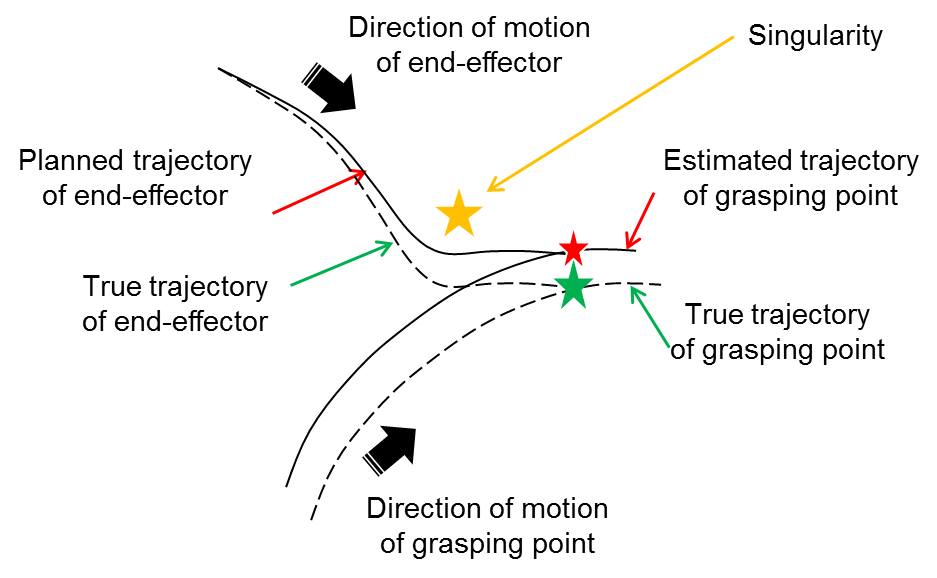
\includegraphics[angle=0,width=0.42\textwidth]{./figures/Motivation_Image}
\caption{The motion of the Target grasping point and of the robot end-effector are shwon for the model-based (solid line) and for the true (dotted line) cases.}
\label{fig:motivation}
%\vspace{-10pt}
\end{figure}
%
\subsection{Problem statement}
% 0.5 pp
%
In the grasping task of interest we assume that the Target has a known geometry, such that model-based computer vision pose estimation can be used. Its angular rate is limited here to 2 deg/s (due to hardware limitations, the limit for the rigidization phase is set to 1 deg/s). %to provide pose estimates between the Target body reference frame and the robot end-effector frame. 
The grasping point on the Target is predefined. %We assume that its motion may be predicted for motion planning purposes [isairas2005] %and is limited in the maximum angular rate modulous to 2 deg./s. (due to hardware limitations, the limit for the stabilization phase is 1 deg/s). %We also assume that the dynamic paratemers of the Target are given with some given level of uncertainty (note that these are identified for motion prediction purposes only to an arbitrary constant [isairas2010]).
%
The Chaser is not actuated (free-floating) and is initially in the same orbit as that of the Target with zero translational and angular velocities relative to the orbital frame.
%space robot consists of a 7 DoF robot manipulator mounted on a free-floating base, the latter not having any GNC actuation active during the task execution. We assume here that the grasping point is in reach of the robot for the complete grasping task. As such, we assume that the Chaser station-keeping has placed the Chaser in the same orbit as that of the Target, in the -V-bar direction, see Fig. ???, with an accuracy of ?? cm, ?? deg., ?? cm/s and ?? deg/sec.. The chaser initially has zero momentum (for the general treatment of the case of non-zero initial momentum see [Ale]).

The grasping task itself is commonly divided into three phases: an approach phase, in which the robot end-effector is brought in the vicinity of the moving grasping point of the Target; a tracking phase, in which the end-effector follows the grasping point with the same velocity, while homing in onto it and closing the grasp; a rigidization phase, in which the relative velocity between the Chaser and the Target is brought to rest by a suitable control of the robot manipulator. 

A feasible trajectory to accomplish this task is provided by a motion planner, first described in~\cite{lampariello2013generating} and extended here. The motion planner relies on a prediction of the Target motion, which can be accomplished as described in~\cite{hillenbrand2005motion}~\cite{aghili2012prediction}. However, in order to complete the task, the tracking controller will initially need to deviate from the reference trajectory, given that the latter is model-based and will differ from the real-world conditions. This fact is shown pictorially in Fig.~\ref{fig:motivation}. Note that the gross motion of the motion planner is still maintained, in order to avoid motion constraints such as, for example, a singularity. 

Due to the deviation from the reference trajectory in the approach and tracking phases, the reference trajectory for the rigidization phase is adapted online, such that the deviation in joint space is recovered. This favours the fullfillment of joint position related constraints (collisions avoidance, singularity avoidance) throughout it. 
%
%It remains to be shown, as we do here, that the reference trajectory can be used by a tracking controller to accomplish the complete grasping task, to include the stabilization. The assumption is in fact that errors in the reference trajectory for the approach phase are sufficiently small. 
%
%If not, the reference trajectory for the stabilization phase may become unfeasible. In fact, while in the approach phase the visual servoing takes care of the necessary trajectory motification, in the stabilization phase, the robot joint controller returns to the reference trajectory, in order to ensure that joint position related constraints (collisions avoidance, singularity avoidance) are fullfilled throughout it. More wil be said about this in Section ???.
%
%In this way, by grossly tracking the reference trajectory the feasibility of the complete maneuver is guaranteed. As such, the end time of the stabilization phase need not be minimal, as suggested in [Aghili], since it is sufficient that the system remains in the vicinity of the planned trajectory, and may be chosen following a different cryterion. Minimum energy maneuvers can be considered as a viable alternative, since, as we will see, they are more robust to modelling errors and visual servo inaccuracies.
%
%Since we also want to be able to deal with a contingency case, for which an undesired impact between the robot and the Target may occur (CHECK need to demonstrate in experiments?), the feedback control method is based on impedance control. This allows to handle the case of an impact robustly, by suitably tuning the impedance []. Furthermore, the possibility of losing the Target after the impact is further greatly reduced by the visual servo.
%
%The aim of the experimental validation includes testing and analysis of the vision guidance (pose estimation), the robot planning, the robot controller, as well as taking imperfect attitude control and robot manipulator control into account. Differently to other works of this kind cited above, due to the macro-micro kinematic structure of our facility, we can include all these elements together in one test environment. Last but not least, the realistic nature of the uncertainty is enhanced in the experimental setup, by the latters's time discretization, time delays, kinematic modelling errors, etcetera. 
%
%Motivation for VS: uncertainty coming from motion prediction (+/- 10 cm in real system), LUT approximation (i.e. solution for desired point is not exact, but how much?), robot model uncertainties (<1 cm), robot controller positioning error (+/- 2 cm), GNC positioning error (+/- 5 cm), GNC velocity error (+/- ? cm/s - see DEOS), unmodelled disturbances (?) - need a scaling rationale: test sum of erros on 3m long robot to see what joint error is to be expected and scale error here accordingly, accounting fr nonlinearity, or validate tests in simulation just as much + look for trajectories for which this error is least visible in joint space!
%
%\section{Robot autonomy and on-orbit servicing}
%
%It is interesting to realize that, as mentioned in Section ??, two different control approaches are foreseable for the grasping task: the telepresence-based and the autonomy-based approaches. The dibate whether one can supersede the other is still open, since both have their benefits and flaws. The first can make use of the operator's intelligence, to include promptness in dealing with unexpected operational conditions and more robustness to adverse lighting conditions. At the same time, the benefit brought by a delayed force reflection (between 30ms and 600ms, for direct and Geo Relay links respectively) to an operator on ground, when executing the grasping of a tumbling Target, is still being investigated upon. Evidence of the difficulty for humans to generally perform this task is already provided in [Aghili's x2], although these used position-controlled robots with low controller sampling rates (check).
%
%On the other hand, autonomous systems are often favoured in industry-driven studies (see for example DEOS and eDeorbit) because of different reasons: the high bandwidth requirements of telepresence (DEOS); the fact that the round-trip-time needs to include the operator reaction time, typically taken to be one second, which in the case of a contingency during grasping may be decisive (eDeorbit); the communication window is limited in the case of a direct link, by the limited ground station coverage, as well as by the possibility of occlusion brought about by the same tumbling Target; communication through a geostationary relay satellite may pose hard challenges in the antenna pointing task, if the Chaser is in synchronized flight with the Target (eDeorbit); finally, the autonomous mode guarantees feasibility with respect to the non-intuitive stabilization task, which was not addressed in the telepresence approach to date.
%
%+ see arguments from Aghili in favour of autonomy.
%
\section{Methods}
\label{sec:methods}
%
In this Section we present the methods used to solve the grasping task, to include elements of the motion planning, the visual-servo with manipulator dynamics, used in the approach and the tracking phases and the joint-position-based tracking control used in the rigidization phase. The control system architecture is shown in Fig.~\ref{fig:blockdiagram}.
%
\begin{figure*}
\psfrag{text_tr}[cc][cc][\FontFigS]{\textbf{Tracking}}
\psfrag{text_st}[cc][cc][\FontFigS]{\textbf{Rigidization}}
\psfrag{text_vs}[cc][cc][\FontFigS]{Visual Servo}
\psfrag{text_pd}[cc][cc][\FontFigS]{\small{\begin{tabular}{@{}l@{}} Compliant\\Controller\\(PD+nullspace\end{tabular}}}
\psfrag{text_pl}[cc][cc][\FontFigS]{\small{\begin{tabular}{@{}l@{}} Plant\\(Chaser\\+manipulator\\dynamics\end{tabular}}}
\psfrag{text_mp}[cc][cc][\FontFigS]{{\begin{tabular}{@{}l@{}} Motion\\Synthesizer \end{tabular}}}
\psfrag{text_js}[cc][cc][\FontFigS]{\small{\begin{tabular}{@{}l@{}} Joint-space\\Rigidization\\controller \end{tabular}}}
\psfrag{t1}[cc][cc][\FontFigS]{\small{\begin{tabular}{@{}l@{}} Camera\\Vision \end{tabular}}}
\psfrag{t2}[cc][cc][\FontFigS]{\small{\begin{tabular}{@{}l@{}} EKF\\Observer \end{tabular}}}
\psfrag{txt_k}[cc][cc][\FontFigS]{\small{\begin{tabular}{@{}l@{}} Kinematics\\(Base/manipulator) \end{tabular}}}
\psfrag{t4}[cc][cc][\FontFigS]{\small{$\begin{bmatrix}q(t_g)\\ \dot{q}(t_g)\end{bmatrix}$}}
\psfrag{EKF_out}[cc][cc][\FontFigS]{\small{$\hat{H}_{eg}$}}
\psfrag{cam}[cc][cc][\FontFigS]{\small{$H_{eg}$}}
\psfrag{ts}[cc][cc][\FontFigS]{\small{$10$ [Hz]}}
\psfrag{t_3}[cc][cc][\FontFigS]{\small{$\tau_{rig}$}}
\psfrag{mp_car}[cc][cc][\FontFigS]{\small{$\begin{bmatrix}H_{eg,ref}\\ \dot{X}_{eg,ref}\end{bmatrix}$}}
\psfrag{t_5}[cc][cc][\FontFigS]{\small{$\begin{Bmatrix}\dot{X}_{e} & \dot{q} & H_{e}(H_b, q) & q\end{Bmatrix}$}}
\psfrag{mp_joint}[cc][cc][\FontFigS]{\small{$\begin{bmatrix}q_{ref}\\ \dot{q}_{ref}\end{bmatrix}$}}
\psfrag{vs_out}[cc][cc][\FontFigS]{\small{$\begin{bmatrix}H_{e,des}\\ \dot{X}_{e,des}\end{bmatrix}$}}
\psfrag{cc_out}[cc][cc][\FontFigS]{\small{$\begin{bmatrix}\tau_{cart}\\ \tau_{null}\end{bmatrix}$}}
\psfrag{int}[cc][cc][\FontFigS]{$\int$}
\psfrag{V_e}[cc][cc][\FontFigS]{\small{$\dot{X}_e$}}
\psfrag{H_e}[cc][cc][\FontFigS]{\small{$H_e$}}
\psfrag{j}[cc][cc][\FontFigS]{\small{$\begin{bmatrix}q\\ \dot{q}\end{bmatrix}$}}
\psfrag{H_T}[cc][cc][\FontFigS]{\small{$H_t$}}
\centering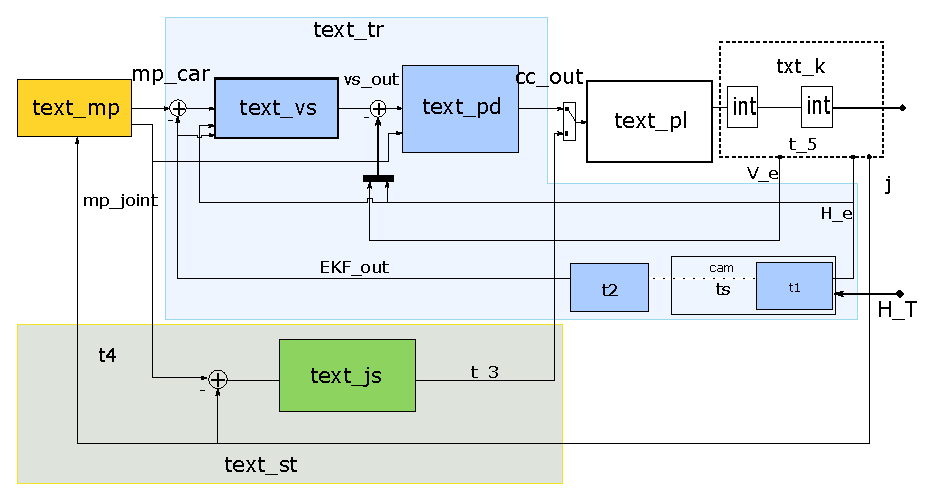
\includegraphics[angle=0,width=0.85\textwidth]{./figures/BlockDia11}
\caption{Control system architecture for tracking or rigidization controllers.}
\label{fig:blockdiagram}
\end{figure*}
%
%\begin{figure*}
%\centering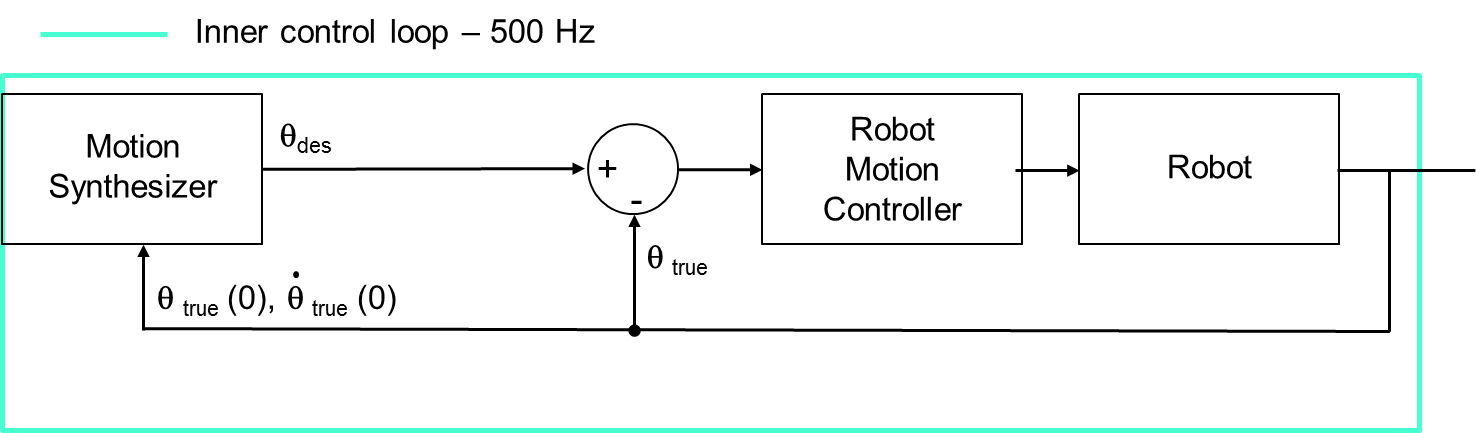
\includegraphics[angle=0,width=0.95\textwidth]{./figures/Block_diagram_stabiliz}
%\caption{Control block diagram for the stabilization phase.}
%\label{fig:blockdiagram2}
%\end{figure*}
%
%\subsection{Control system architecture - 0,5 pp}
%
%A block diagram of the control systems for the approach and tracking phase and for the stabilization phase are shown in Fig.~\ref{fig:blockdiagram} and Fig.~\ref{fig:blockdiagram2} respectively. 
%
%\subsubsection{Plant}
%The plant refers to the free-floating robot, consisting of a free-floating satellite base and a 7 DoF robot manipulator. The only actuators present are those of the robot joints, since the base is assumed to be non-actuated. The sensors include the position and torque sensors of the robot joints and a stereo-camera at the robot end-effector. The satellite states are assumed to be ideal (check).
%
%Define reference frames. inertia, body, end-effector, other.
%
%\subsubsection{Target}
%This block represents the simulation of the Target motion, including that of the predefined grasping point on it.
%
%\subsubsection{Motion synthesizer}
%The motion synthesizer receives the reference trajectory from the motion planner and interpolates the desired Cartesian pose and robot configuration in time. Note that this function runs on-board of the Chaser spacecraft, whereas the reference trajectory is generated on ground before the task is executed.
%
%\subsubsection{Robot controller and forward kinematics}
%This is the inner loop of the robot controller, which runs at a sampling time of 1KHz. It containts two elements to control both the Cartesian pose and the joint configuration in null space. The forward kinematics provides the current Cartesian pose of the robot end-effector through a forward kinematics computation. The robot controller then, based on the chosen control strategy (see Section ??), determines the control torques to be applied to the robot. The satellite states are assumed to be ideal (check).
%
%\subsubsection{Camera-based motion estimation}
%This block represents the computer vision algorithm which runs onboard at a slower sampling rate of 10Hz and which provides the current relative pose between the robot end-effector and the Target grasping point (check). 
%
%The connections between these blocks constitute the visual servo and will be addressed in Section ?? in detail.
%
\subsection{Motion planning and motion synthesizer}
% - 1 pp
%
\subsubsection{Approach and tracking phases}
The free-floating dynamics of the robot manipulator are given by~\cite[\S 55]{siciliano2016springer}
\begin{equation} \label{eq_manip_main}
  \begin{bmatrix}
    \mathbf{M}_b &     \mathbf{M}_{bm} \\     \mathbf{M}_{bm}^T &     \mathbf{M}_m  \end{bmatrix} \begin{bmatrix}
    \ddot{\mathbf{x}}_b\\ \ddot{\mathbf{q}}\end{bmatrix} + \begin{bmatrix}     \mathbf{C}_b &     \mathbf{C}_{bm} \\     \mathbf{C}_{mb} &     \mathbf{C}_m \end{bmatrix} \begin{bmatrix}
    \dot{\mathbf{x}}_b\\ \dot{\mathbf{q}} \end{bmatrix} = \begin{bmatrix}
    0\\ \mathbf{\tau}
    \end{bmatrix}
\end{equation}
where $    \mathbf{M}_b \in \mathbb{R}^{6\times 6}$, $    \mathbf{M}_{bm} \in \mathbb{R}^{6\times 7}$, $    \mathbf{M}_m \in \mathbb{R}^{7\times 7}$ are the locked, coupled and $7$-joint manipulator's inertias respectively. $\mathbf{C}_b \in \mathbb{R}^{6\times6}, \mathbf{C}_{bm} \in \mathbb{R}^{6\times7}, \mathbf{C}_{mb} \in \mathbb{R}^{7\times 6}, \mathbf{C}_m \in \mathbb{R}^{6\times7}$ make up the whole Coriolis matrix, $\mathbf{\tau} \in \mathbb{R}^7$ are the joint torques, $\dot{\mathbf{x}}_b \in \mathbb{R}^6$ is the twist of the base and $\mathbf{q} \in \mathbb{R}^7$ are the joint positions respectively. 
The motion planning \rev{problem relating to the approach and tracking phases is formulated as a point-to-point task (with non-zero final velocity) and an inverse differential kinematics task to follow it~\cite{lampariello2013generating}. Mathematically, the first step can be formulated as the constrained optimal control problem
\begin{equation}
\min_{\MatO{q}_1(t)} \Gamma{}_1(\MatO{q}_1(t))
\end{equation}
subject to 
\begin{equation}
\MatO{M}_{b}\: \MatO{\ddot{x}_{b}} \:+ \:\MatO{C}_{b}\:\MatO{\dot{x}_{b}}\: + \:\MatO{C}_{bm}\:\MatO{\dot{q}}=\:-\MatO{M}_{bm} \: \MatO{\ddot{q}{}_1}
\label{eq:dyn}
\end{equation}
\begin{equation}
\MatO{h}{}_1(\MatO{q}{}_1, \MatO{\dot{q}{}_1}) \le 0
\label{eq:const3}
\end{equation}
for $0\le t \le t_f{}_1$ and to the boundary conditions
\begin{equation}
\MatO{f}{}_1(\MatO{H}_e(t_f{}_1))=0, \: \MatO{g}{}_1(\MatO{x}^e(t_f{}_1))=0
\label{eq:const5}
\end{equation}
\begin{equation}
\MatO{q}_1(0)=\MatO{q}_1{}_{in}, \MatO{\dot{q}}{}_1(0)=0.
\label{eq:const1}
\end{equation}
(\ref{eq:dyn}) then is an equality constraint stemming from the first line of these equations with a term on the right-hand side for rheonomically driven joints. $t_f{}_1$ is a predefined relative final time. $\Gamma{}_1$ is a predefined cost function. $\MatO{h}{}_1$ include inequality box constraints of type $\MatO{x}_{min} \le \MatO{x}(t) \le \MatO{x}_{max}$, for $\MatO{x}=\{\MatO{q}{}_1, \MatO{\dot{q}}{}_1 \}$.

Functions $\MatO{f}{}_1$ and $\MatO{g}{}_1$ are equality constraints on the final end-effector pose $\MatO{H}_e(t_f{}_1)$ and twist $\dot{\mathbf{x}}_e(t_f{}_1)$ to be in a desired relative non-zero position and orientation with respect to the grasping point and travelling at its velocity. (\ref{eq:const1}) expresses boundary conditions on position and on velocity. 

The cost function is chosen to be the mechanical energy of the robot manipulator, in order to smoothen the solution, i.e.
\begin{equation}
\MatO{\Gamma} = \int^{t_f{}_1}_{0} (\MatO{\tau}_1{}^{T}(t) \: \MatO{\dot{q}}_1(t)){}^2 dt.
\label{eq:cost}
\end{equation} 

The tracking phase consists of an inverse differential kinematics solution, which is dictated by the motion of the Target. Its duration is defined by the relative time $t_f{}_2 - t_f{}_1$. The same motion constraints apply for this phase as for the previous. During this phase, a constant homing-in velocity brings the end-effector onto the grasping point, closing the gap due to the non-zero relative position at the end of the previous phase. The solution is expressed by $\MatO{q}{}_2(t)$.
} 

The method in~\cite{lampariello2013generating} is extended here to account for the requirements stemming specifically from the visual tracking. It is in fact required that throughout the approach phase sufficient features of the Target are in view of the camera (e.g., the Target's solar panel on its top suface) and that the pixel velocity in the image remains low. These result in motion constraints, the first of which is treated with an inequality constraint on the pitch angle $\phi{}_{e}$ of the end-effector frame $\mathcal{E}$ \rev{(rotation about its $y$-axis) CHECK} relative to the target frame $\mathcal{T}$ (see Fig.~\ref{fig:facility}), defined as
\begin{equation}
\phi{}_{e}{}_2 \leq \phi_{e \: mid}{}_2 + \phi_{e \: delta}{}_2,
\end{equation}
where $\phi_{e \: mid}$ is a parameter to define a middle value for $\phi{}_{e}$ and $\phi_{e \: delta}$ is a paremeter which relates to the field-of-view of the camera. 

Defining the pixel velocities in the $x$ and $y$ components of the end-effector frame $\mathcal{E}$ to be ${}^{e}v{}_{px}={}^{e}v{}_{y}{}^{te}\ / {}^{e}r{}_{z}{}^{te}$ \rev{and ${}^{e}v{}_{py}={}^{e}v{}_{x}{}^{te}\ / {}^{e}r{}_{z}{}^{te}$}, inequality constraints are also introduced as
\begin{eqnarray}
-\Delta {}^{e}v{}_{px}  \leq {}^{e}v{}_{px} \leq \Delta {}^{e}v{}_{px} \\ 
-\Delta {}^{e}v{}_{py}  \leq {}^{e}v{}_{py} \leq \Delta {}^{e}v{}_{py},
\end{eqnarray}
where $\Delta {}^{e}v{}_{px}$ and $\Delta {}^{e}v{}_{py}$ are parameters which relate to the pixel velocity limits in the camera image. Note that the velocity constraint in~\ref{eq:const5}, not present in~\cite{lampariello2013generating}, contributes to minimizing the pixel velocity, by minimizing the relative velocity between the robot end-effector and the Target.

The output of the motion planner is judiciously defined to account for two important aspects. Firstly, a reference trajectory of the end-effector is provided relative to the grasping point frame $\mathcal{G}$ on the Target, i.e., as homogeneous trasformation $\MatO{H}{}_{ge, ref}(t)$ and twist $\MatO{\dot{x}}{}_{ge, ref}(t)=[{}^{g}v^{ge} \: {}^{g}\omega^{ge}]{}^T(t)$, for $0 \le t \le t_f{}_2$. Note that the end-effector pose is effectively given by $\MatO{H}{}_{ge}=\MatO{H}{}_{gI}\MatO{H}{}_{Ie}$. The tracking controller is designed to track this relative motion. This ensures that any error in $\MatO{H}{}_{gI}$ (Target motion prediction errors) and in $\MatO{H}{}_{Ie}$ (tracking control errors, robot forward kinematic errors) are intrinsically eliminated in following the desired relative motion $[\MatO{H}{}_{ge, ref}](t)$, which is independent of these uncertainties. Note however, that the motion of the robot relative to absolute space, and therefore joint space, will deviate from the motion planning solution. This relates to the second aspect to be considered, namely that a reference trajectory is also provided in the joint space of the robot manipulator, $[\MatO{q}{}_{ref}, \MatO{\dot{q}}_{ref}](t)$. As will be shown in Section~\ref{sec:approach_control}, the tracking control law contains a main term to minimize the Cartesian tracking error and a second term, projected in the null-space of the robot manipulator, to minimize the tracking error in joint space (see (\ref{eq:control_law}) and (\ref{eq:control_law_2})). This is intended to minimize the deviation of the robot motion in joint space from the feasible reference trajectory. The null-space term also cares for the kinematic redundancy of the robot manipulator. 

%The motion planner cannot run online, due to its computational runtimes and to the lack of strict guarantees on convergence time. The motion synthesizer, which runs online, interpolates the outputs defined above, namely $[\MatO{H}{}_{eg, ref}{}_{i}, \MatO{V}{}_{eg, ref}{}_{i}], q_{ref}{}_{i}$, for $0 \leq i\leq N$, where $N$ is the number of output steps of the motion planning solution. 
%
\subsubsection{Rigidization phase}
\label{sec:rigidization}
%
The rigidization phase requires bringing the robot joints velocity to zero, while ensuring that the motion constraints are not violated. We solve
\begin{equation}
\min_{\MatO{q}{}_{3}(t)} \Gamma{}_{3}(\MatO{q}{}_{3}(t))
\end{equation}
subject to 
\begin{equation}
\MatO{M}_{b\:mod}\: \MatO{\ddot{x}_{b}} \:+ \:\MatO{C}_{b\:mod}\:\MatO{\dot{x}_{b}}\: + \:\MatO{C}_{bm\:mod}\:\MatO{\dot{q}}=\:-\MatO{M}_{bm\:mod} \: \MatO{\ddot{q}{}_1}
\label{eq:dyn_mod}
\end{equation}
\begin{equation}
\MatO{q}(t_{0}{}_{3})=\MatO{q}(t_f{}_1+t_{f}{}_{2}),
\MatO{\dot{q}}(t_{0}{}_{3})=\MatO{\dot{q}}(t_f{}_1+t_{f}{}_{2})
\label{eq:const2_3}
\end{equation}
\begin{equation}
\MatO{\dot{q}}(t_{0}{}_{3}+t_{f}{}_{3})=\MatO{0}
\label{eq:const2_4}
\end{equation}
\begin{equation}
\MatO{h}{}_{3}(\MatO{q}{}_{3}(t)) \le \MatO{0}
\label{eq:const3_3}
\end{equation}
where the initial conditions in (\ref{eq:const2_3}) express the dependency on the final conditions of the previous tracking phase. The matrices $\MatO{M}{}_{b\:mod}$, $\MatO{M}_{bm\:mod}$, $\MatO{C}_{b\:mod}$ and $\MatO{C}_{bm\:mod}$ of the free-floating robot dynamics are updated to include the inertial properties of the Target on the end-effector.

In this phase, the offline motion planner provides a reference trajectory in joint space. The  tracking controller here is a joint space controller. The task is to rigidize the compound after the grasp, bringing the relative motion between the two satellites to zero. Given that only internal forces come into play, the angular momentum of the Target is shared with the Chaser and at the end of the maneuver the two satellites tumble with a new angular velocity, function of their total inertia. The cost function is chosen to be the mechanical energy of the robot manipulator, as in~(\ref{eq:cost}), in order to minimize its loads on the joints and on the end-effector. \rev{Due to the small Target tumbling velocities considered, it was found that these loads are very low and do not require relative motion constraints.}
%\begin{equation}
%\MatO{\Gamma} = \int^{t_{rf}}_{t_{ri}} (\MatO{\tau}{}^{T}(t) \: \MatO{\dot{q}}(t)){}^{2} dt
%\label{eq:cost}
%\end{equation}
%where $t_{ri}$ $t_{rf}$ are the initial and final times of the motion. 

%
\rev{
\subsubsection{Method for the contrained optimization problem}

The optimization problem described above is solved as a nonlinear programming problem (NLP). The inequality constraints $\MatO{h}$ are satisifed at a finite number of $k$ via points. The equality constraints in ~(\ref{eq:dyn}) and ~(\ref{eq:dyn_mod}) are satisfied by numerical integration. As such, the NLP is solved with a single shooting approach, with parameterization of the joint positions in time, i.e., $\MatO{q}_i=\MatO{q}(t,\MatO{p}_i)$, where $\MatO{p}_i$ is a column matrix containing $\text{N}_i$ optimization parameters and $i$ is either 1 or 3. For the approach and for the rigidization problems described above, two parameter sets $\MatO{p}{}_1$ and $\MatO{p}{}_{3}$ result. The NPL is solved with the Sequential Quadratic Programming algorithm from the MOPS library~\cite{MOPS_1}. The numerical integration is performed with an explicit fifth order Runge-Kutta method. }

In the online setting however a modification of the reference trajectory for the ridigization is necessary, to account for the deviation from the reference trajectory in the previous approach phase. Each joint trajectory is parameterized with a uniform B-spline, the parameters of which are the optimization parameters to be found. The solution parameters generated offline are still used to synthesize online a new rigidization trajectory, by modifying them with the measured initial robot manipulator joint states. Let the measured initial position and velocity for a given joint be $q_{0m}$ and $\dot{q}_{0m}$ respectively, and the B-spline parameters $q_i, 1 \leq i \leq N_B$ ($N_B<N$ and $N-N_B$ are the parameters which satisfy the boundary conditions). The modified parameters are then taken to be:
\begin{equation}
q_{i \: mod} =   q_i +  \left( q_0 - q_{0m} + \frac{\dot{q}_{0m} \: ({t_{rf}}-{t_{ri}})}{N_B} \right) \: \frac{(N_B-i)}{N_B},
\end{equation}
where the second term accounts for the initial position deviation $q_0 - q_{0m}$ and the joint velocity at the initial time times the duration of the first B-spline segment, $({t_{rf}}-{t_{ri}})/N_B$, in which the spline cannot be modified. This effectively smoothly brings the joint configuration back to the one planned offline. As such, the fullfilment of the joint position related motion constraints is favoured. The chosen modification of the trajectory could however give rise to an increase in robot joint torques, since it implies pushing the Target onto the predicted trajectory. Note however, that the choice of the cost function and of $t_{rf}$ in Eqn.~(\ref{eq:cost}) minimize these, allowing for a larger margin from their limits.
%
%The optimization problem for the stabilization phase was treated in a similar way as the approach phase. The joint states were parameterized with B-slines and provided the initial conditions in position, velocity and acceleration (check) resulting at the end of the tracking phase. The final conditions on the joint states were only expressed for the joint velocities and accelerations, leaving the joint positions open for the optimizer to be determined, in function of the assigned cost function. Note that this point solves an open issue when only implenting a dissipating control law, to stabilize the compound. In fact, doing so firstly does not give any bound on the final position reached at the end of the motion and as such no guarantee that collisions are avoided. Secondly, due to noise in the system, a purely dissipative control law results in a continuously drifting system (check with Marco and add results later?). The number of parameters was increased, for better convergence performace. 
%
%Of notice here is also to realise that the choice of parameterizing the robot joints was favoured with respect to that of parameterizing the end-effector trajectory. This is firstly because the robot control needs joint position commands, which in our case are given directly from the solution, without having to revert to an inverse kinematics function, to great advantage of the motion synthesizer (see Section ??). The use of an inverse kinematics function is also generally not advisable for the case that a singularity is met (location not known and function of inertia distribution). In this case, the inverse of the Jacobian is undefined. However, we note that singulatities also provide numerical problems in the presented formulation, due to the fact that even in their vicinity, the joint velocities increase noticeably. The integration of the equations of motion of a free-floating system is very sensitive to large velocities, leading the necessity of an excessively small integrator step size. Check - show example in results?
%
%With regars to the cost function, we chose here to minimize the mechanical energy. We propose it as alternative to minimizing the end time given that we track the solution in joint position and as such guarantee the collision avoidance that could arise from any residual relative drif velocity between the two spacecrafts. Although minimizing the mechanical energy requires defining a final time, since the solution would otherwise push the end time to infinity, an arbitrary sensible value can be chosen by the user, after inspection of the first solutions. It is important to stress that the goal of the motion planner is first to provide a feasible solution. The optimality is then used to make the solutions more robust to the uncertainties. Finally, due to the highly nonlinear nature of the problem (check), a global search is performed, in order to find a (close to) global minimum for a given query. Although we do not address the task of generating a look-up table here, for any tumbling state of interest, we revert the reader to [IROSD2013] for further details on this point.
%
%21/12/2017: the chosen cost function for the rigidization is the integral of the product $tau*qd$. This is best to option to reduce the effort of the LBR! Only drwaback is that is does not look nice, i.e. the target rotates toward the chaser (did a global search and could not find any better solutions). The integral of the product $F_e*v_e$ could be an interesting alternative (given that it implies a solution where the target slows down along its path, without rotating toward the chaser) to minimize the risk of collision, although we can deal with that.
%
%
%End of current version
%
%
%Explain motion synthesizer - give details of on-line B-spline with on-line modification function of new robot joint states + Phillip, Marco + see how this can work on board for all required outputs to controller! Then explain how Cartesian trajectory could be modified with motion prediction during approach and how resulting cartesian reference trajectory could be perfectly updated to real motion (relative to the base body). But must chose to give preference to joint position error (which neglects target trajectory change, otherwise don't know where will end up) and possible collision avoidance or to Cartesian error and possible end-effector and joint torque error (show how this can grow, for a given trajectory error!). As such minimizing energy gives a smooth solution and as such a more robust solution to prediction errors, since far from the motion boundaries and not on the edge of them (optimal handling of uncertainties on the off-line generated motion plannign solutions). Favoured here avoiding singularities. Furthermore, say that for LBR on OOS-SIM 5 cm error are a lot, but for 3/4 m long arm not. 
%
%Say that: The presented method needs to be able to meet strict guarantees on the solution (such as the upper bound on the computation time), for the safety-critical application at hand (software ceritifcation processes also need to be considered). As such, all computations involving optimization algorithms have to be performed off-line on ground. 
%
%0. motion planning (Roberto):
%	v. say that opt. params for Chaser position are very important for good convergence properties - but add params in approach to improve convergence - to do!
%	vi. say about minimizing joint motion or joint motion in null-space for approach phase - see use of nullspace term in invkin (see dkin2!!!) - to reduce effect of friction in NS dynamics of real robot - talk to Christian.
%	vii. say that for LBR on OOS-SIM 5 cm error are a lot, but for 3/4 m long arm not.
%	viii. compare min energy solution to solution from $F_e=K_d * Deltax_dot$ (must implement), for different Chaser/Target mass ratios
%	ix. do global search for min energy or command given $v_e, omega_e$ to inv-kin to see solution
%	x. add $q_ddot$($tf_approach$) as parameters to minimize tau($0_tracking$)
%	xi. compare joint space to cartesian space stabilization solution approaches
%	x. the problem of extracting the optimal solution from the LUT is not addressed in any more detail here (see IROS 2013)
%
%In pp method?
%In the proposed method, a motion planner provides a reference trajectory to execute the task described above, details of which can be found in [IROS2013]. Of notice it the fact that the method in [IROS2013] is meant to firstly guarantee the feasibility of the task with respect to all motion constraints, described in Section??. This differes from any of the approaches described in Section???, since there many important constraints are either not treated exhaustively (e.g., joint position and velocity, the latter in view of dynamic singularities, the position of which for a ff 3D system with n dof and with load X on e-e cannot be predefined to date), implying that the explicit effect of a disturbance or uncertainty on the future evolution of the system is not taken into account, or only added in the cost function as a weighting term (e.g., line-of-sight of end-effector cameras, for which the useful Target features may be lost, with obviously negative consequences), thus not guaranteeing their fullfillment. Here instead, the method based on nonlinear optimization, guarantees the fullfillment of the constraints for the reference trajectory (at the chosen via points, of arbitrary number, sufficient for the task). Due to the highly non-linear nature of the problem, the presented method also provides a (near to) global optimimum, for a very wide range of cost functions, for example,  minimized for improvement of the robustness of the control method, to model uncertainties and sensor errors, by performing a global search for a given task. The method finally allows to represent the system in question in its full free-floating dynamic behaviour, without the need to reduce the Chaser dynamics to those of a fixed-based robot, for ease of resolution of the related optimal control problem. We will see in Section ??? that the stabilization task is in fact a momentum transfer problem, rather than a detumbling (or passivation?) problem, with useful consequences on the resulting solutions found. The tumbling of the compound after the stabilization is by no means an issue, when realizing that the minimization of the attitude has been solved with simple technological solutions, such as omnidirectional antennas and gymbal joints [DEOS]. The impelling need for robot autonomy for the grasping task was also made evident in [eDeorbit], underlining the need for full autonomy, for which a communication link in the critical grasping phase is not foreseen.
%+ In the same Figure, the necessity for a motion planner is underlined by showing how this deviates around a robot singularity, rather than going right through it, as a simple regulation controller would do.
%+ make clear statements about singularities: although inv kin methods can avoid them, we can't tell if the motion after them is then feasible anymore, given non-holonomic nature of Chaser dynamics + if cannot avoid them right during tracking, we have a problem + cannot represent them yet.
%+ The uncertainties are quantified and analysed here to some extent, to validate the truthfullness of the assumption. 
%+ This last point has required making a decision between prioritizing position related to force related constraints. The internal forces required for the adjustment of the trajectory in the stabilization phase are function of the tracking error in the approach phase, and as such unknown. The alternative would be to recompute the stabilization trajectory online in cartesian space and tranfer the unknown onto the final position reached by the robot... 
%+ The feasibility (region) is provided by the motion planner, not by the user [Aghili's ball]. 
%	
%
%
\subsection{Extended Kalman Filter (Model-based control)}
The Extended Kalman Filter (EKF) is a ubiquitous state observer for nonlinear systems. It is a nonlinear observer in the sense that the model propagation is nonlinear whereas, the error injection is linear. In the context of this paper, the EKF provides robustness to the tracking controller against incoming measurement outliers from the computer vision algorithm by ensuring measurement continuity. Due to its predictor-update structure, it also provides a state prediction which allows us to compensate for image-processing time-delays and ensure continuous control errors during occlusion or measurement failures caused by degenerate observability conditions. From a tracking controller perspective, the EKF also estimates the target velocities for a feed-forward term for the Visual Servo, which compensates for the disturbance due to target motion that acts on the controller.

\rek{\begin{assumption} \label{ass_ignore_clw}
Since the scope of this paper is limited to an operational time, $T < 20$ [sec], the contribution of the term which accounts for the relative translation due to orbital motion, and is given by the Clohessy-Wiltshire equations, is neglected.
\end{assumption}}
The dynamic system \rek{for the EKF} is modeled with the state, \rek{$x_a \in \mathbb{R}^{13} = \begin{bmatrix} \theta^T& r^T& \omega^{b^T}& \dot{r}^T&\end{bmatrix}^T$} as,
\begin{align}
\frac{d}{dt}\begin{bmatrix} \dot{\theta} \\ r \\ \omega^b \\ \dot{r}\end{bmatrix} = \begin{bmatrix}\frac{1}{2}\omega^b \otimes \theta \\ \dot{r} \\-\omega^b_\times I\omega^b \\ \Phi(n) \end{bmatrix}        \label{eq_SysDyn}
\end{align}
where $\otimes$ denotes the quaternion multiplication tensor, $(.)_\times$ denotes the skew-symmetric form of $\mathbb{R}^3$. $\Phi(n)$ is the linear approximation of orbital dynamics given by the Clohessy-Wiltshire equations \rek{\cite{Aghili07}} for mean anomaly $n$. Based on ass.~\ref{ass_ignore_clw}, $\Phi(n) = \mathbf{0}_{3,3}$.

\rek{For the quaternion group, $Q$, in the multiplicative variant of the EKF, the quaternion state is maintained as a $3$-component vector as $\delta \theta(a_p) \in T_{\overline{\theta}}Q$, at a nominal value of the quaternion $\overline{\theta}$. $T_{\overline{\theta}}Q$ is the tangent space to the quaternion manifold and $a_p$ is a 3-component parameterization vector.} A detailed \rek{discussion} on such vector expressions was given in \cite{Markley}. In this text, the Modified Rodriguez Parameters (MRP), $a_p$ was chosen \rek{so that singularity is not encountered before angular error $2\pi$}. \rek{The tangent vector $\delta \theta$, the parameterization vector $a_p$ and the quaternion $\theta$ are related as follows},
\begin{align}
\rek{a_p(\theta) = \frac{4}{1+\theta_0}\theta_v}\quad,
\rek{\delta \theta_v(a_p) = \frac{1}{16}\begin{bmatrix}
8a_p \\ 16 - a_p^Ta_p
\end{bmatrix}}
\end{align}
The differential form for $a_p$ is given as,
\begin{align} \label{eq_quat_kin}
\dot{a}_p = \Big(-\frac{1}{2}\omega_\times^b + \frac{1}{8}\Big)a_p + \Big(1 - \frac{1}{16}a_p^Ta_p\Big)\omega^b 
\end{align}


Among the alternatives for scaled inertia parameterization for zero-torque motion propagation, \cite[\S 4.6]{TweddlePhD} the $3$-parameter ($p_x,~p_y,~p_z$) form proposed in \cite{Aghili07} is used. So, the angular dynamics can be \rek{written by reformulating the rotational dynamics Euler equation in eq.~\eqref{eq_SysDyn}} as,
\begin{align} 
 \dot{\omega}^b = \psi(\omega^b) =  \begin{bmatrix}
 p_x \omega_y^b \omega_z^b \\
  p_y \omega_x^b \omega_z^b \\
   p_z \omega_x^b \omega_y^b  
 \end{bmatrix}
\end{align} 
which \rek{has a} linear approximation about the \rek{current} estimate, $\hat{\omega^b}$ \rek{as},
\begin{align} \label{eq_lin_rot_dyn}
	\delta \dot{\omega^b} = \mathbf{M}\delta{\omega^b}
\end{align} where $M = \Big( \frac{\partial \psi(\omega)}{\partial \omega^b}\Big)_{\omega = \hat{\omega^b}}$ is a hollow matrix \cite{Aghili07}.

Finally, \rek{using eq.~\eqref{eq_quat_kin}, \eqref{eq_lin_rot_dyn} and eq.~\eqref{eq_trans_kin_ass} from ass.~\ref{ass_ignore_clw},} the linear approximation of the \rek{torque-free} system \eqref{eq_SysDyn} with state $x \in \mathbb{R}^{12} = \begin{bmatrix}a_p^T&r^T&\omega^{b^T}&\dot{r}^T & \end{bmatrix}$ is given in \cite[eq. 4.79]{TweddlePhD} as,
\begin{align}
\dot{x} = \mathbf{A}x + \mathbf{B}w
\end{align}
From the Fig.~\ref{fig:facility}, the measurement is derived by using current forward kinematics ($\mathbf{H}_e$) and known target geometry ($\mathbf{H}_{tg}$) is given as,
\begin{align} \label{eq_meas_facility}
g = \begin{bmatrix}r\\ \theta\end{bmatrix} = \begin{bmatrix}
R(\eta_c)^T r_c + \rho_c -R(\eta_t)\rho_t\\ \eta_t^*\otimes\mu\otimes \eta_c \end{bmatrix}
\end{align}
\rek{where $(.)^*$ refers to the quaternion inverse.}
In order to obtain the EKF measurement $y$ from available measurement$g$, $a_p$ is computed from eq.~\eqref{eq_meas_facility}.
The linear approximation for the EKF measurement was \rek{derived several times before in \cite{Aghili07}, \cite{Dubowsky}, \cite{TweddlePhD}, and we only state the final formula as,}
\rek{\begin{align}
y = \mathbf{H}x,~\mathbf{H} = \begin{bmatrix}
- R(\overline{q})\rho_{t_\times} & 0_{3,3} & 1_{3,3} & 0_{3,3}\\
 1_{3,3} &   & & 0_{3,9}
\end{bmatrix}
\end{align}}
\rek{where $\mathbf{H} = \frac{\partial y}{\partial x} \Big|_{x_a = \hat{x}_a}$ is obtained by linear approximation of the measurement function about the current state estimate $\hat{x}_a$}. Since the Kalman Filter equations are standard, we do not explicitly write the prediction-update form. The interested reader is referred to \cite{Kalman} for seminal paper on equations. By using the aforementioned system of equations, the EKF was implemented with the Outlier-rejection (OR) scheme suggested in \cite{Selfpaper} to provide robustness against local outliers from the vision system. \rek{The EKF output $\hat{y} = \begin{bmatrix}\hat{r_c}^T & \hat{\mu}^T\end{bmatrix}^T \equiv \hat{\mathbf{H}}_{eg}$ is used for control in the next step.}
%
\subsection{Visual Servo for Approach and Tracking Phases}
\label{sec:approach_control}
\rek{
For the free-floating space manipulator, eq.~\eqref{eq_manip_main} can be reformulated after eliminating terms explicitly depending on $\mathbf{x}_b$ and its derivatives as, 
\begin{equation}\label{eq_reduced_dyn_js}
 \hat{\mathbf{M}}_m(\mathbf{q},\mathbf{x}_b)\ddot{\mathbf{q}} + \tilde{\mathbf{C}}_m(\mathbf{q},\dot{\mathbf{q}},\mathbf{x}_b,\dot{\mathbf{x}}_b)\dot{\mathbf{q}} = \mathbf{\tau},  \quad \text{(free-floating model)}
\end{equation}
where $\hat{\mathbf{M}}_m = \mathbf{M}_m - \mathbf{M}_{bm}^T\mathbf{M}_b^{-1}\mathbf{M}_{bm}$, $\hat{\mathbf{C}}_b = \mathbf{C}_{mb} - \mathbf{M}_b^{-1}\mathbf{C}_b$, $\tilde{\mathbf{C}}_m= \hat{\mathbf{C}}_m(\mathbf{q},\dot{\mathbf{x}}_b,\dot{\mathbf{q}}) - \hat{\mathbf{C}}_b(\mathbf{q},\dot{\mathbf{x}}_b,\dot{\mathbf{q}})\mathbf{M}_b^{-1}\mathbf{M}_{bm}$, are the generalized terms (see \cite{Nech_Yosh_ff}) and $\hat{\mathbf{C}}_m = \mathbf{C}_m - \mathbf{M}_b^{-1}\mathbf{C}_{bm}$. Using the formulation in \cite[eq. 10]{Ott}, the eq.~\eqref{eq_reduced_dyn_js} can be written only for the Cartesian dynamics as, 
\begin{equation}
\mathbf{\Lambda}_m(\mathbf{q},\mathbf{x}_b)\ddot{\mathbf{x}}_e + \mathbf{\mu}_m(\mathbf{q},\dot{\mathbf{q}},\mathbf{x}_b,\dot{\mathbf{x}}_b)\dot{\mathbf{x}}_e = \mathcal{\mathbf{F}}_e
\end{equation}
where $\mathbf{\Lambda}_m = (\mathbf{J}_g(\mathbf{q},{\mathbf{x}}_b)\hat{\mathbf{M}}_m^{-1}\mathbf{J}_g(\mathbf{q},{\mathbf{x}}_b)^T )^{-1}$, $\mathbf{\mu} = \mathbf{J}_g(\mathbf{q},{\mathbf{x}}_b)^{-T}\tilde{\mathbf{C}}_m\mathbf{J}_g(\mathbf{q},{\mathbf{x}}_b) + \mathbf{J}_g(\mathbf{q},{\mathbf{x}}_b)^{-T}\hat{\mathbf{M}}_m\frac{d}{dt}\mathbf{J}_g(\mathbf{q},{\mathbf{x}}_b)^{-1}$ where $\mathcal{\mathbf{F}}_e$ is the Cartesian control torque.}


\rek{In the context of On-Orbit Servicing, the target is partially cooperative in that its model is available in advance. As a result, \rek{in this paper, the kinematic-level control used is Position-based Visual Servo (PBVS), which means that the control law uses the pose error $\hat{\mathbf{H}}_{eg}$ that is reconstructed from image-space measurements}. Based on the model-based visual tracking and EKF's \rek{pose} results, this control law is used to provide a desired velocity ($\hat{\dot{X}}_e$) and pose for the inner loop impedance controller. }

\rek{In accordance to fig.~\ref{fig:blockdiagram}, a kinematic tracking velocity for the manipulator is generated using the visual servo law. Firstly, the reference trajectory is used to compute a desired end-effector pose $\mathbf{H}_{e,des} = (\mathbf{H}_e\hat{\mathbf{H}}_{eg}) \mathbf{H}_{ge,ref}$. Secondly, this function is used as a pose error to construct the visual servo law $\hat{\dot{\mathbf{x}}}_e =\begin{bmatrix}\dot{r}_e^T  &\omega_e^T\end{bmatrix}^T$. Using the slow-sampled $\hat{\dot{\mathbf{x}}}_e$, a virtual frame is generated by integrating $\dot{\mathbf{H}}_{e,v}(R_{e,v},p_{e,v})$. Note here that this virtual frame is solved as an initial value problem between two EKF sampling times and acts like an intermediate trajectory for the manipulator between these sampled points. This is initialized as, $\mathbf{H}_{e,v}(n) = \mathbf{H}_e(n) ~\forall n \in [1..k]$ where $n$ is the $n^{th}$ EKF sample time. The control law used is, 
\begin{equation} \label{eq_VS_law}
\begin{split}
 \hat{\dot{\mathbf{x}}}_e &= K_1 e_{pose}(H_{e,v},~H_{e,des}) + \mathbf{v}_t\\
 \mathbf{v}_t &= \begin{bmatrix}\hat{\dot{r}} \\ R(\hat{\mu})\hat{\omega}^b \end{bmatrix}
 \end{split}
\end{equation}
where $k_{1,ii} > 0, ~\forall~ i \in [1...6]$, $e_{pose}$ is the pose error function defined as, $e_{pose}(H_1,H_2) = \begin{bmatrix}(p_1-p_2)^T& \psi(R_1^TR_2)^T\end{bmatrix}^T$, with the rotation error $\psi(R) = \frac{1}{2}[R - R^T]^\vee$ and $[a_\times]^\vee = a, ~a\in \mathbb{R}^6$ is the mapping from skew symmetric matrix to vector form. $\mathbf{v}_t$ is simply the estimated Target velocity applied as a feed-forward. A note on this error formulation and subsequent Lyapunov function analysis can be found in \cite{BULLO199917}.}

\rek{
Finally, a compliant controller is placed in cascade after the visual servo which acts upon the Cartesian error. The impedance error is a Cartesian error observed in the inertial frame and is denoted as $\mathbf{e} = e_{pose}(\mathbf{H}_{e,des},\mathbf{H}_e)$. Using the corresponding velocity error $\dot{\mathbf{e}}$, a PD+ Cartesian control law is formulated as,

\begin{align}
\mathbf{\mathcal{F}}_m = \mathbf{\Lambda}_m(\mathbf{q},\mathbf{x}_b) \hat{\ddot{\mathbf{x}}}_e + \mathbf{\mu}_m(\mathbf{q},\dot{\mathbf{q}},\mathbf{x}_b,\dot{\mathbf{x}}_b) \hat{\dot{\mathbf{x}}}_e - \mathbf{K}_P\mathbf{e} - \mathbf{K}_D\dot{\mathbf{e}}
\end{align}
where $k_{P,ii} > 0$ and $k_{D,ii} > 0, ~\forall~ i \in [1...6]$ are the choices for Cartesian stiffness and damping terms respectively.}
The corresponding joint torques with null-space control torque $\mathbf{\Gamma}$ are given as,
\begin{equation}
\mathbf{\tau} = \mathbf{J}_g^T\mathbf{\mathcal{F}}_m + (\mathbf{1}_{n,n}-{\mathbf{J}_g}^T\mathbf{J}_g^{*^T})\mathbf{\Gamma}
\label{eq:control_law}
\end{equation}
where $\mathbf{J}_g^{*}$ is the dynamically consistent Weighted Pseudo-inverse of $\mathbf{J}_g$ (generalized Jacobian) and $\Gamma$ is given by
\begin{equation}
\Gamma = -\MatO{K}_{PN} (\mathbf{q} - \mathbf{q}_{ref}) - \MatO{K}_{DN}  (\dot{\mathbf{q}} - \dot{\mathbf{q}}_{ref} )
\label{eq:control_law_2}
\end{equation}
\rev{where the two terms on the right hand side are a stiffness and damping terms respectively, with constant diagonal gain matrices $\MatO{K}_{PN}$ and $\MatO{K}_{DN}$.}

~\rev{In eq.~\ref{eq:control_law_2}, the two terms on the left hand side are a stiffness and damping terms for the null-space respectively, with constant diagonal gain matrices $\MatO{K}_{PN},~k_{PN,ii} > 0$ and $\MatO{K}_{DN},~k_{DN,ii} > 0, ~\forall~i \in [1...7]$. 

Note that the use of $ \MatO{J}_{g}$ ensures that the Cartesian and null-space coordinates are decoupled in the inertia matrix. However Coriolis/Centrifugal matrix remains coupled \cite[eq. 10]{Ott}. This coupling is argued in \cite[pp. 2001]{Ott} to be of minor importance in practice. The validity of the reference trajectory guarantees that the null-space projection in eq.~\ref{eq:control_law} is not null. However, as shown in Fig.~\ref{fig:motivation}, uncertainties in the reference trajectory require departing from it in inertial space, but not relative to the target. As such, the null-space term will not converge but only minimize the error as $\text{min}_{f(q) = \mathbf{H}_{e,des}}||\mathbf{q} - \mathbf{q}_{ref}||_2$, where $f({q})$ is the forward kinematics function.}

%
%
%
% Hrishik
% Describe rational and method (equations) of visual servo
% Describe KF method, refer to existing literature (ASTRA?)
%
% Roberto
% Describe LWR impedance controller
% Describe null-space controller
%
%1. Control Visual Servo Approach (Hrishik, Roberto)
%        -i. describe how to command the planned trajectory to the visual servo (optimization offline on ground, what is done on-line on board?), such that it is grossely followed, both in Cartesian and in joint space, but at the same time corrected by the feedback controller, to account for modelling errors and other uncertainties.
%	0. The visual servo is described in detail, to include tuning of an inner-loop impedance controller with an outer-loop visual servo, in the approach and tracking phase.
%	i. updated DEOS block diagram (position and impedance control), feedforward term, other
%	ii. inputs from path planner - e-e trajectory, configuration trajectory for null space, other
%	iii. theory for tracking of relative motion
%	iv. theory for tracking of null-space -ask Christian/Alin
%	v. visual servo (computer vision, visual servoing)
%	vi. robot control method for ff robot (Jg) and tracking control; what is maximum allowed impedance of LWR?
%	vii. use of KF with preidentified model parameters, for CV failure (e.g., due to occlusions)
%	viii. The satellite states are assumed to be ideal - check which are needed: $r0, v0, ori_0, omega_0$, sampling time (3 Hz, 1 kHz), other
%	


\subsection{Computer Vision for Approach and Tracking Phases}
%
% Nassir
%
% describe CV method, refer to existing references
% provide analysis to explain why CV fails, with reference to experiemental data (image sequences)
The visual pose estimation is based on work of~\cite{Drummond2002} which relies on a known object geometry. The algorithm consisits of sampling model contours and edge detection, followed by a local optimization of the 3D rigd-body transform. The re-projection error is then minmized to allign visible model contours and image edges using the Levenberg-Marquardt algorithm.
 %Related to this model matching approach is moving edges method~\cite{Comport2004} which differs from the former in contour samply strategy. The latter samples model contours in 2D, after projecting model lines on the image. These two approaches have their own advatnages and disadvantages which have been explored in~\cite{Comport2005}. While both approaches show similar performance, the former is easier to implement as it presents a direct and accurate formulation for minimizing the reprojection error from %3D to 2D~\cite{Oumer2015}. 
The complex tumbling motion of the target poses difficulty in visual tracking. In order to address this problem, a motion prediction scheme based on an extended kalman filter is integrated into the local optimization. The prediction here relies on a simple kinematic motion model, assuming constant frame to frame motion. Under this assumption, the visual tracker is able to cope with a relatively high image motion between two camera frames. Moreover, the short-term prediction scheme helps the visual tracker reduce the search space in order not to remain trapped in potential local optima during minimization of the cost function. \rev{If the tracker does remain trapped (see for example Fig.s~\ref{fig:fig_norm_errors} and~\ref{fig:states_EKF}), the algorithm needs to be reinitialized either with an external global detector or with the EKF presented in Section II.B CHECK. The latter in fact satisfies the realtime constraints and makes use of the dynamic model of the Target. This approach will be implemented in future work.} The qualitative tracking results are illustrated in Fig.~\ref{fig:TrackingImages}, with examplar tracked images from the approach and tracking phases. Those in red indicate the projections of the model contours onto the image edges at the estimated pose. The overlap of the model contours and image edges shows the successful tracking and pose estimation.
%
%\begin{figure}
%\centering
%\begin{subfigure}
%	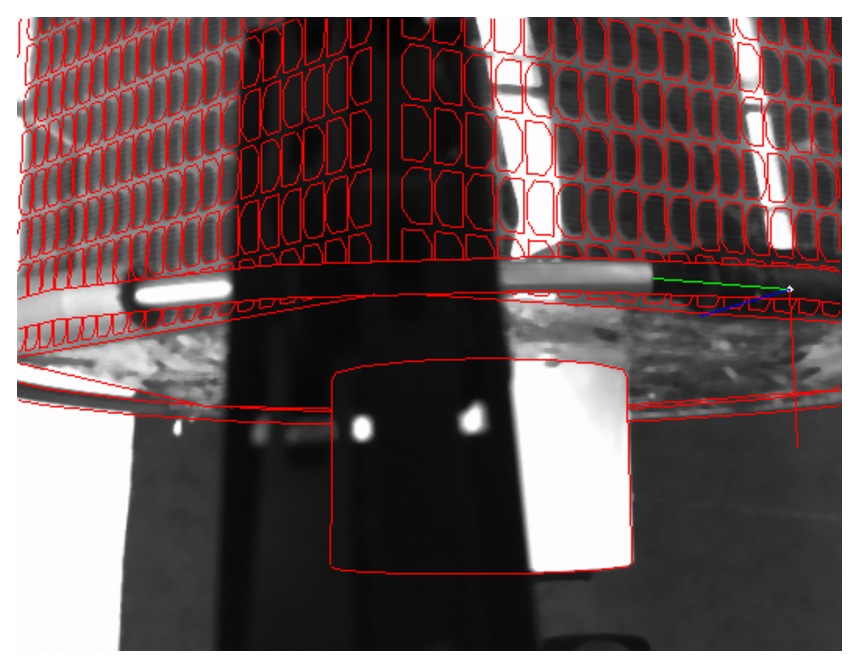
\includegraphics[angle=0,width=0.95\textwidth]{./figures/frame0786_result_cam0}
%	\caption{approach}
%\end{subfigure}
%\begin{subfigure}
%	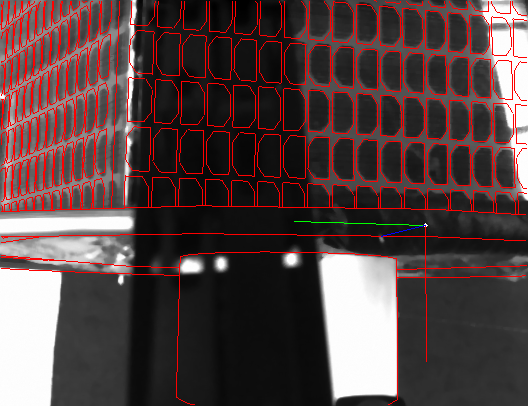
\includegraphics[angle=0,width=0.95\textwidth]{./figures/frame0849_result_cam0}
%	\caption{Tracking}
%\end{subfigure}
%\begin{subfigure}
%	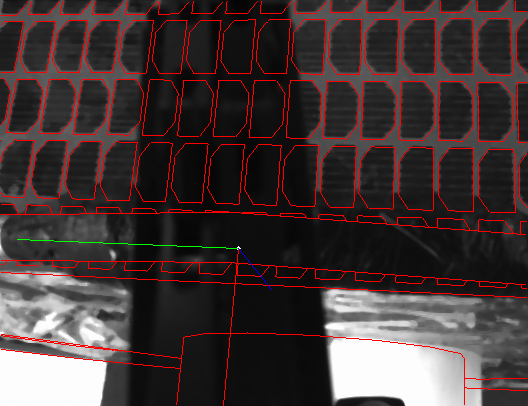
\includegraphics[angle=0,width=0.95\textwidth]{./figures/frame0922_result_cam0}
%	\caption{Tracking}
%\end{subfigure}
%\begin{subfigure}
%	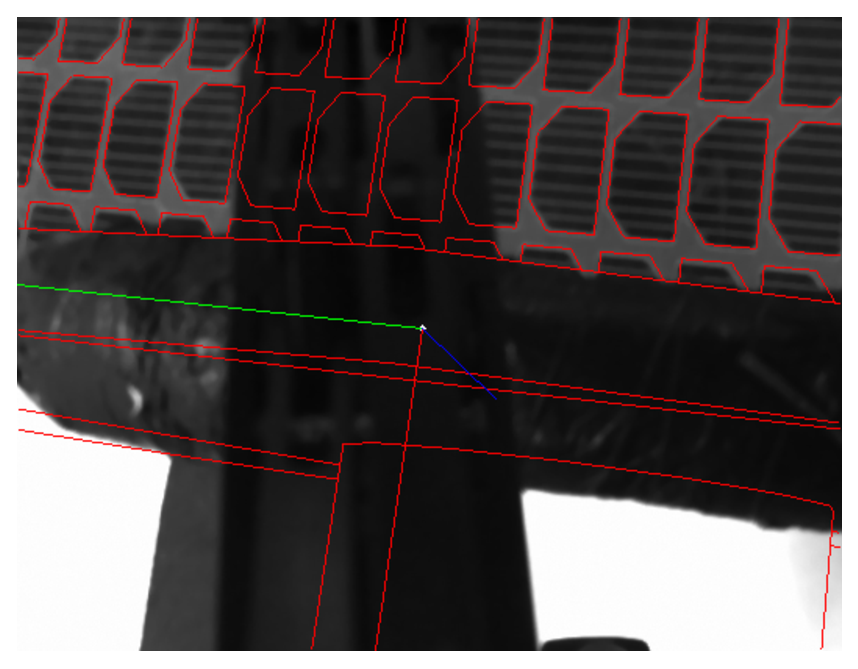
\includegraphics[angle=0,width=0.95\textwidth]{./figures/frame0954_result_cam0}
%	\caption{Tracking}
%\end{subfigure}
%\label{fig:TrackingImages}
%\caption{Exemplar images during visual tracking for approach and tracking phase. The overlay of the model contours and image edges shows the successful tracking and pose estimation. The %target features reduce significantly as the manipulator approaches close to grasping. The axes of the coordinate frame of grasping point is indicated in red, green and blue }
%\end{figure}


%
\begin{figure*}
\centering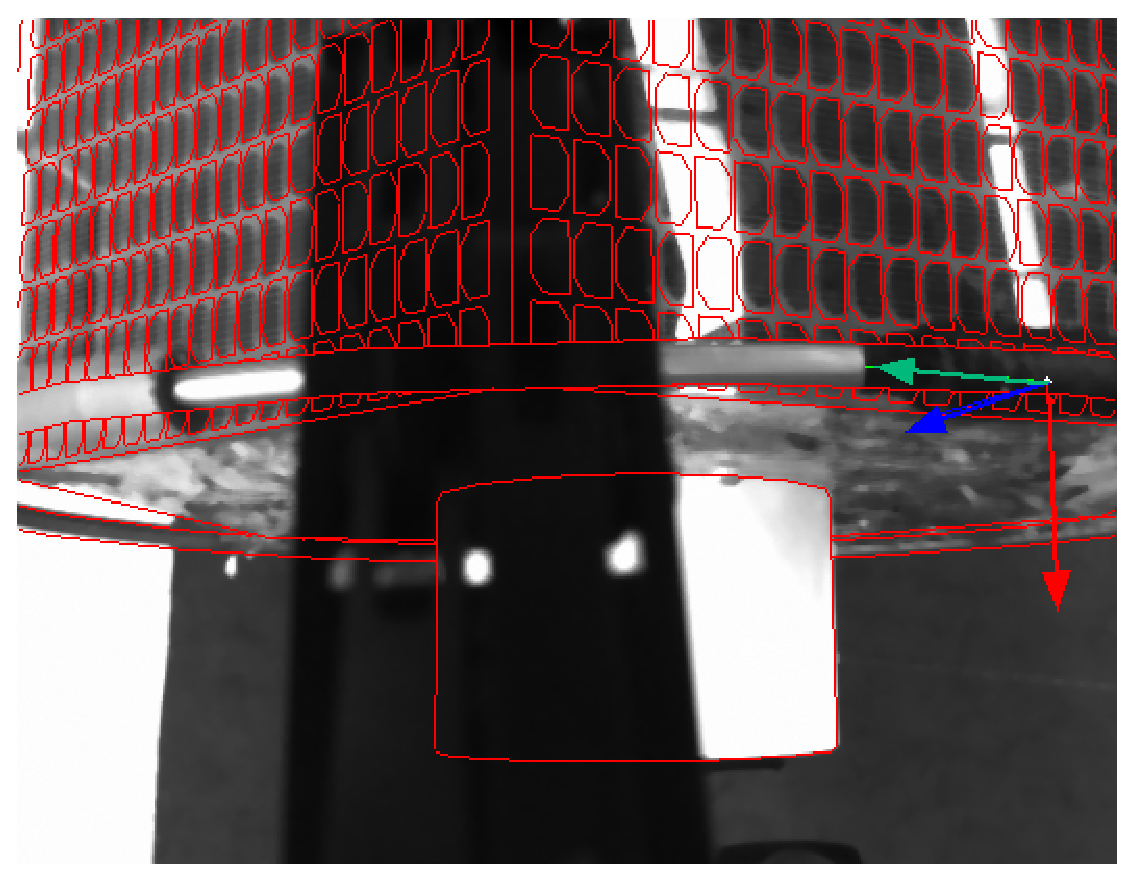
\includegraphics[angle=0,width=0.24\textwidth]{./figures/frame0786_result_cam0_xes}
\centering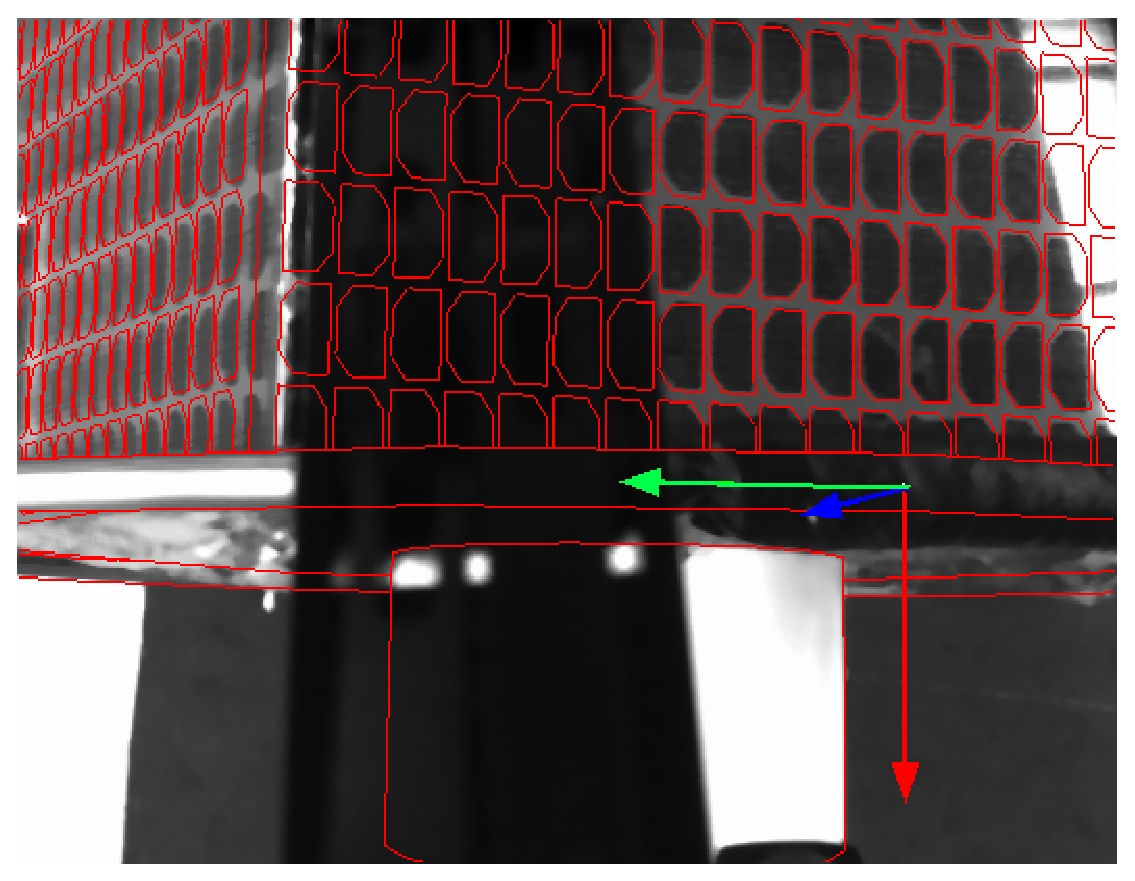
\includegraphics[angle=0,width=0.24\textwidth]{./figures/frame0849_result_cam0_xes}
\centering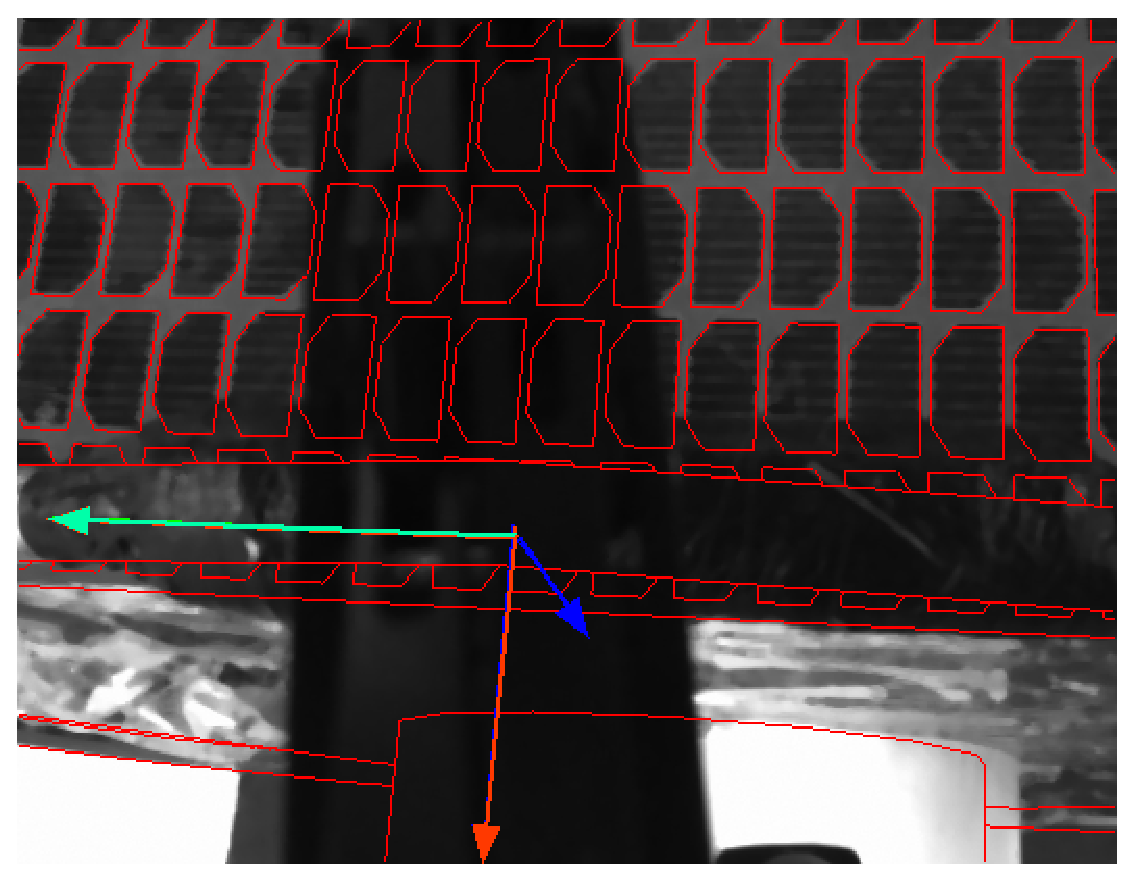
\includegraphics[angle=0,width=0.24\textwidth]{./figures/frame0922_result_cam0_xes}
\centering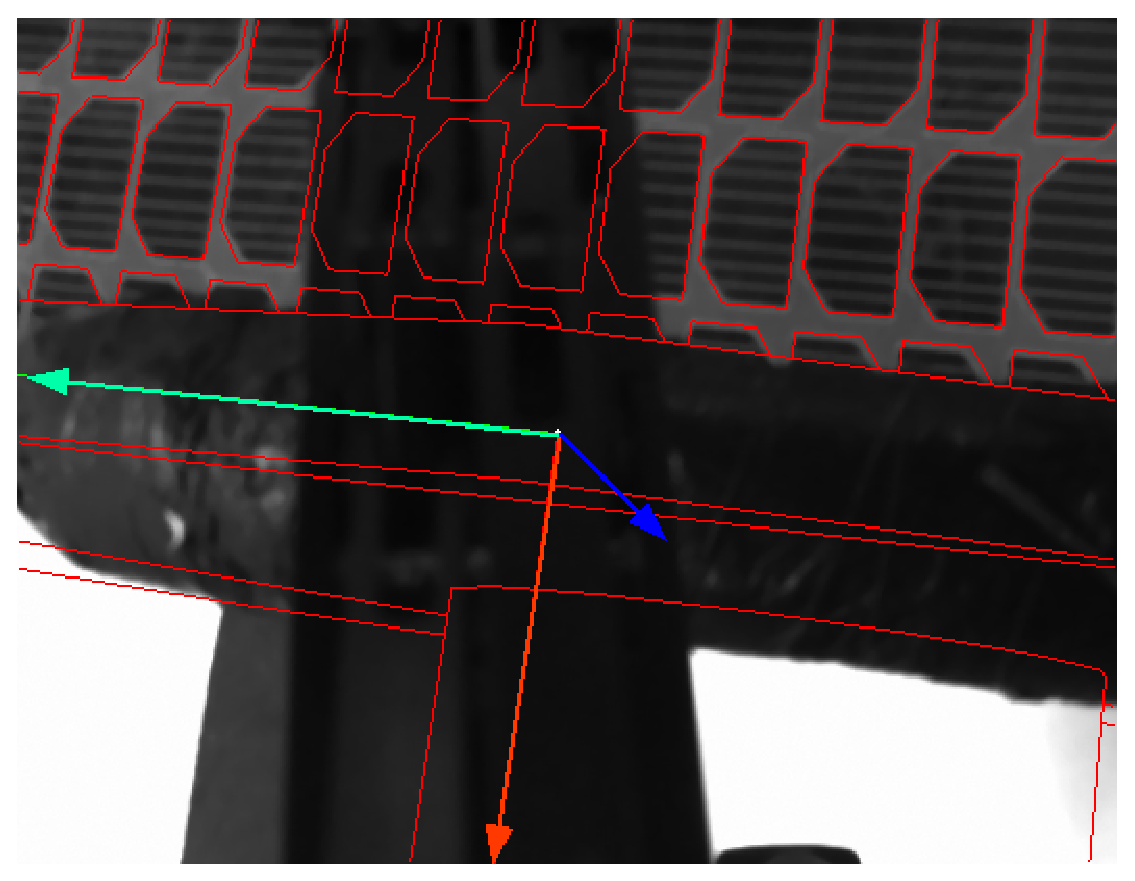
\includegraphics[angle=0,width=0.24\textwidth]{./figures/frame0954_result_cam0_xes}
\caption{Exemplar images during visual tracking for approach and tracking phase. The overlay of the model contours \rev{(in red)} and image edges shows the successful tracking and pose estimation. The axes of the coordinate frame of the grasping point $\{\mathcal{G}\}$ are indicated in red, green and blue. The target features reduce significantly at very close range because of gripper finger occlusion (black in the image) and camera field of view.}
\label{fig:TrackingImages}
\end{figure*}


%There exist, however a few cases where the visual tracking was not able to provide the required pose accuracy for the visual servoing. For example, the inherent vision-based %pose estimation problem assocociated to in-plane motion where lateral rotation estimation error is large, particularly when a partial surface of the target with planar geometry is momentarily visible in non perspective view. Moreover, the outliers due to occlusion and limited field of view poses tracking failure particularly at very close range, as shown in Fig.~\ref{fig:GraspingImages}. Fortunately, at this range the gripper is a few millimeters from the grasping point, hence the implemented motion predictor supports final grasping phase.

%\begin{figure}
%\centering
%\begin{subfigure}
%	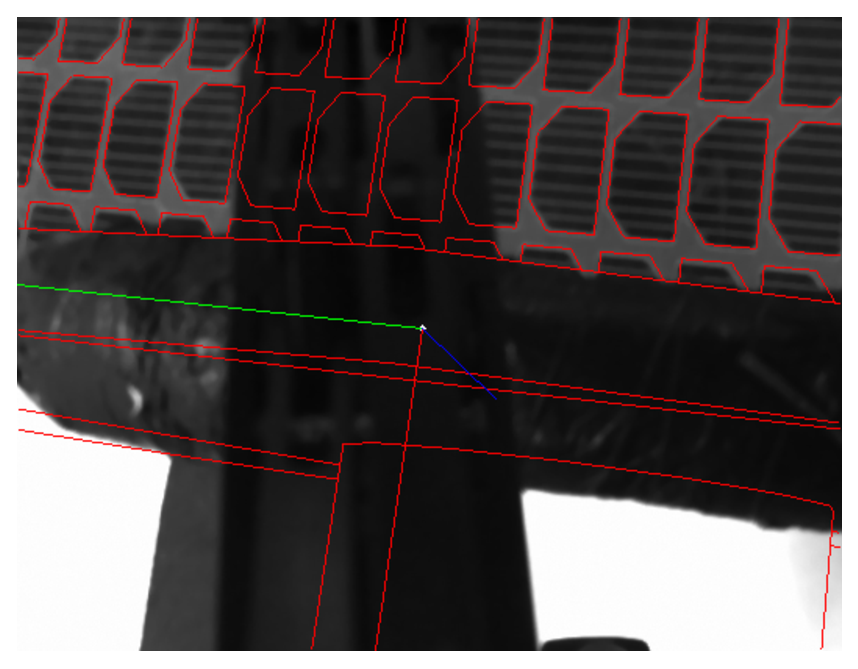
\includegraphics[angle=0,width=0.95\textwidth]{./figures/frame0954_result_cam0}
%	\caption{approach}
%\end{subfigure}
%\begin{subfigure}
%	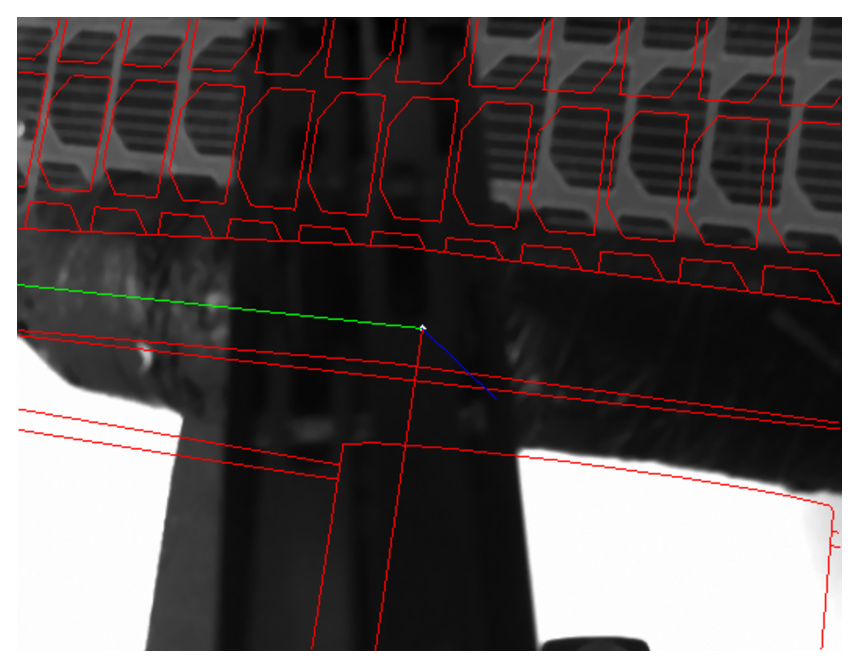
\includegraphics[angle=0,width=0.95\textwidth]{./figures/frame0955_result_cam0}
%	\caption{Tracking}
%\end{subfigure}
%\begin{subfigure}
%	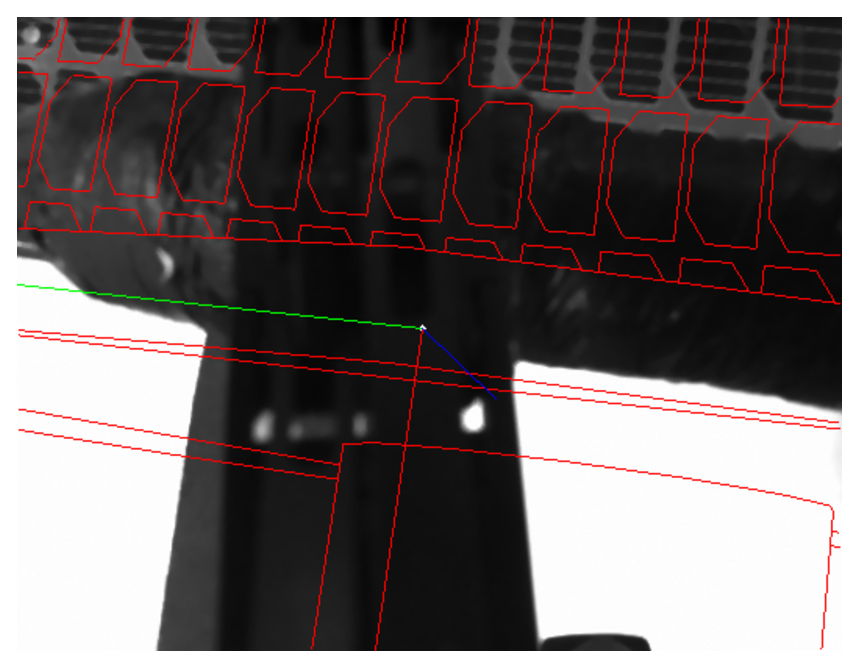
\includegraphics[angle=0,width=0.95\textwidth]{./figures/frame0956_result_cam0}
%	\caption{Tracking}
%\end{subfigure}
%\label{fig:GraspingImages}
%\caption{Failure cases of the visual tracking. At very close range, the visible target features are not sifficient for pose estimation because of occlusion (black in the images) and  %reduced field of view}
%\end{figure}

%\begin{figure*}
%\centering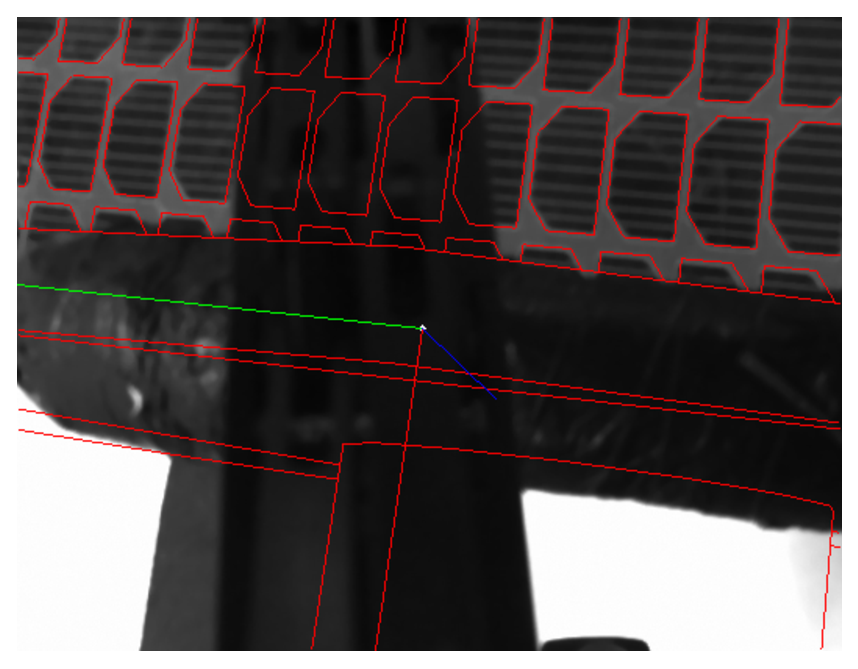
\includegraphics[angle=0,width=0.24\textwidth]{./figures/frame0954_result_cam0}
%\centering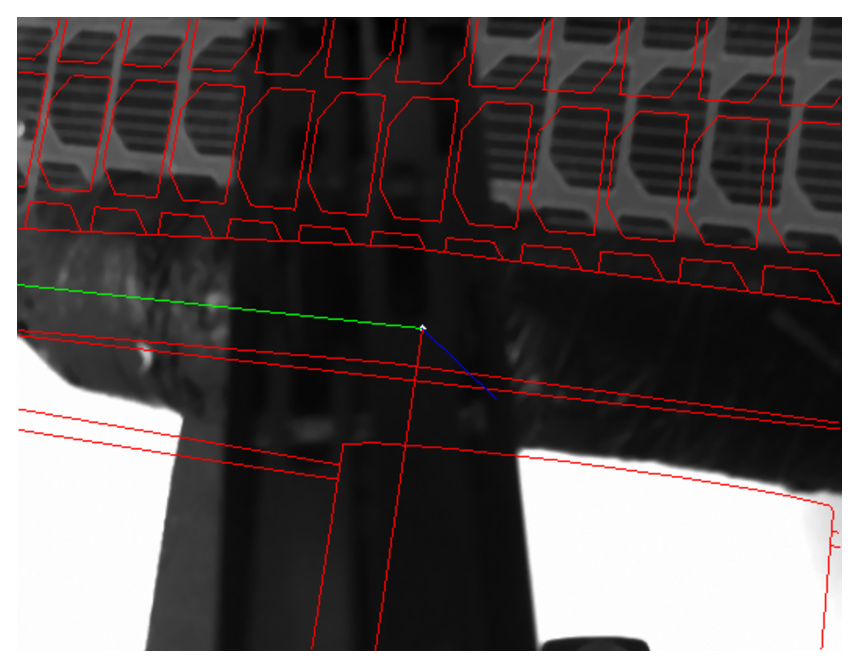
\includegraphics[angle=0,width=0.24\textwidth]{./figures/frame0955_result_cam0}
%\centering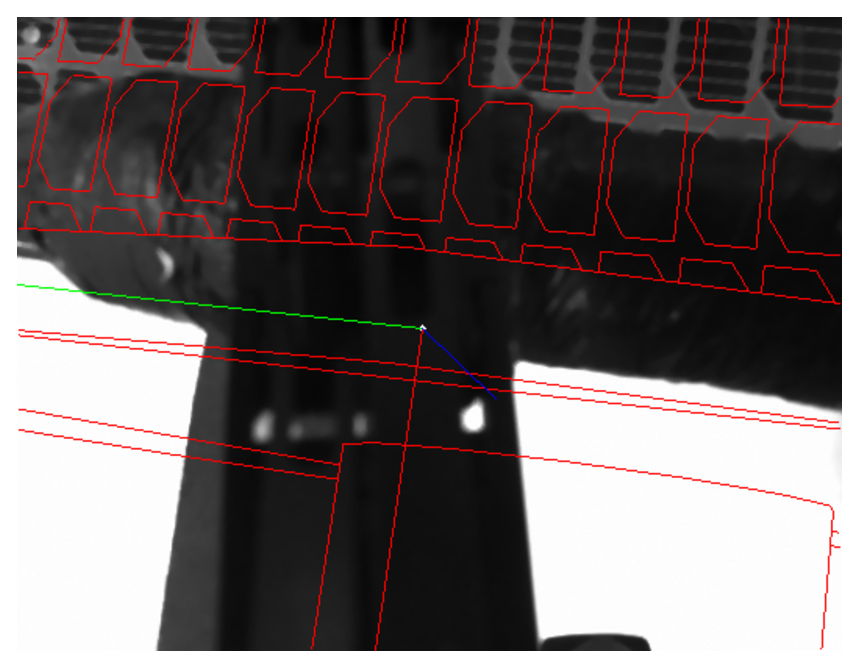
\includegraphics[angle=0,width=0.24\textwidth]{./figures/frame0956_result_cam0}
%\caption{Failure cases of the visual tracking. At very close range, the visible target features are not sifficient for pose estimation because of occlusion (black in the images) and  reduced field of view.}
%\label{fig:GraspingImages}
%\end{figure*}

% ---- You may menstion this in future work section-----
%In the future, the performance of the visual tracking will be improved, addressing problems related to in-plane motion, local minima and large image pixel velocity by integrating dynamic motion model of the coupled satellite-manipulator system for long-term prediction. Moreover, the visual tracking will be validated in a representative space environment with proper lighting conidtion as in~\cite{OumerPhdThesis}.

%	i. The visual servo also includes a pose estimation algorithm, which relies on a predefined simplifies model of the Target - show image with simplified model of the target

%
\subsection{Joint Tracking Control for Stabilization Phase}
%
% Roberto or Marco
% Describe tracking controller
% 
The tracking controller for the rigidization phase is described in Fig.~\ref{fig:blockdiagram}. The motion synthesizer provides an input expressed as $q_{r}, \dot{q}_{r}$. \rek{The PD+ control law for the tracking controller \cite{Paden} adopted here is then as follows}
\rek{
\begin{equation}
\begin{split}
\MatO{\tau}{}_{rig} =& \hat{\mathbf{M}}_{m,t}(\mathbf{q},\mathbf{x}_b)\ddot{\mathbf{q}}_{r} +  \tilde{\mathbf{C}}_{m,t}(\mathbf{q},\dot{\mathbf{q}},\mathbf{x}_b,\dot{\mathbf{x}}_b)\dot{\mathbf{q}}_{r}\\ &+ \MatO{K}{}_{p} (\mathbf{q}_{r}-\mathbf{q}) + \MatO{K}{}_{d} (\dot{\mathbf{q}}{}_{r}-\dot{\mathbf{q}})
\label{eq:rigidiz_control}
\end{split}
\end{equation}}
where $\MatO{K}{}_{p}, ~k_{p,ii} > 0$ and $\MatO{K}{}_{d},~k_{d,ii} > 0, ~\forall~i = [1..7]$ are (7x7) diagonal matrices including the stiffness and damping gains respectively and\rek{, $\hat{\mathbf{M}}_{m,t}$ and $\tilde{\mathbf{C}}_{m,t}$ are inertia and Coriolis matrices computed by adding the transformed target inertia to $\hat{\mathbf{M}}_m(\mathbf{q},\mathbf{x}_b)$ and $\tilde{\mathbf{C}}_m(\mathbf{q},\dot{\mathbf{q}},\mathbf{x}_b,\dot{\mathbf{x}}_b)$ respectively from eq.~\eqref{eq_reduced_dyn_js}. Note that, this is based on the assumption that the target CoM is the new end-effector frame}. The \rek{third} proportional term plays an \rek{important} role, since it brings the system into a feasible final configuration, as dictated by the motion planner. 
 
 


%
%
%
%
\section{Experimental facility}
% Roberto
%	i. introduce falicity
%	ii. describe extensions: target motion, post-grasping tumbling motion
%	iii. 4N/1Nm (CHECK) deadband in Target FTS - removed after grasping
%	iv. End-effector pads to avoid slipage (?)
%
The OOS-SIM experimental facility is described in detail in~\cite{7139588}. %Some new features were implemented to perform the grasping task of a rotating Target. The motion of the Target was allowed in all of its six degrees of freedom, by means of the online integration of its equations of motion (single rigid body) and the input to this from a force/torque sensor at the base of the Target mockup. Due to the sensor noise and to uncertainty in the gravity compensation of the sensor signal for the mockup weight (approx. 30 kg), a deadband filter was used in the approach and tracking phase in all three Cartesian directions. The filter was however removed at the moment of gripper closure and for the subsequent rigidization phase.
%
\rev{However, in order to simulate the motion of the two satellites after the grasp, a new approach was used, based on the conservation of momentum. We note, in fact, that after the grasp the forces of interaction between the Target and the Light-Weight Robot (LWR CHECK) are internal and, as such, do not alter the total momentum of the Chaser-LWR-Target system. Based on the measured relative pose between the Target and the LWR, the dynamic model of the Chaser-LWR multibody system is updated at the time of grasping (end of closure of gripper), $t_{ri}$,  to modify the inertial properties of the LWR's end-effector, to include those of the Target. From this point on, the laws of conservation of momentum are integrated in time, in function of the measured LWR joint positions and their first derivatives, as follows. Given the relationship between the twist of the Chaser $\MatO{\dot{x}}{}_{e}$ and the velocity of the LWR robot joints as~\cite{siciliano2016springer}}
\begin{equation}
\MatO{M}{}_{b} \MatO{\dot{x}}{}_{e} + \MatO{M}{}_{bm} \MatO{\dot{q}} = \MatO{L}
\label{eq:mom_cons}
\end{equation}
\rev{where $\MatO{L}$ is the constant total momentum, we first note that the latter is assumend to be zero before the grasp. At $t=t_{stab}$, matrices $\MatO{M}{}_{m}$ and $\MatO{M}{}_{bm}$ are modified to include the modelling of the Target. The left-hand side is also updated to be equal to the measured momentum of the Target. Assuming that there is no impact at the grasp, the current state of the system is then valid as initial conditions for integrating Eq. CHECK~(\ref{eq:mom_cons}) in $\MatO{\dot{x}}{}_{e}$, i.e.,}
\begin{equation}
\int_{t_{ri}}^{t_{ri}+t} \MatO{\dot{x}}{}_{e} \: \text{d}t = \int_{t_{ri}}^{t_{ri}+t} \MatO{M}{}_{b\;mod}^{-1} \left( \MatO{L}{}_{mod} -  \MatO{M}{}_{bm\;mod} \: \MatO{\dot{q}} \right) \: \text{d}t
\end{equation}
\rev{which provides the pose $\MatO{H}{}_{e}$ to be commanded to the OOS-SIM industrial robot which simulates the Chaser. The Target was then commanded to followed the Light-Weight Robot through the internal actions which the latter imparted on it. These, as done in~\cite{7139588}, were sensed by the FTS at the base of the Target and given as input to the online integration of its equations of motion.}

\rev{With this approach we do not use the FTS of the Chaser to determine its motion, as done in~\cite{7139588}, thus eliminating sources of simulation error. In fact, the FTS signal is affected by modelling errors (since the signal has to be corrected by the LWR gravity term) as well as by drift (due to sensor noise). We still use the FTS to determine the motion of the Target, since the inaccuracy of the forward kinematics of the facility does not favour a position control approach.}
%
%
%
%
%
%
\section{Results}
\label{sec:results}
%
%
%
%
% 1 pp
%
\begin{figure}[t!]
\psfrag{qd}[cc][cc][\FontFigB]{$\MatO{\dot{q}}$ [deg/s]}
\psfrag{t}[cc][cc][\FontFigB]{$t$ [s]}
\centering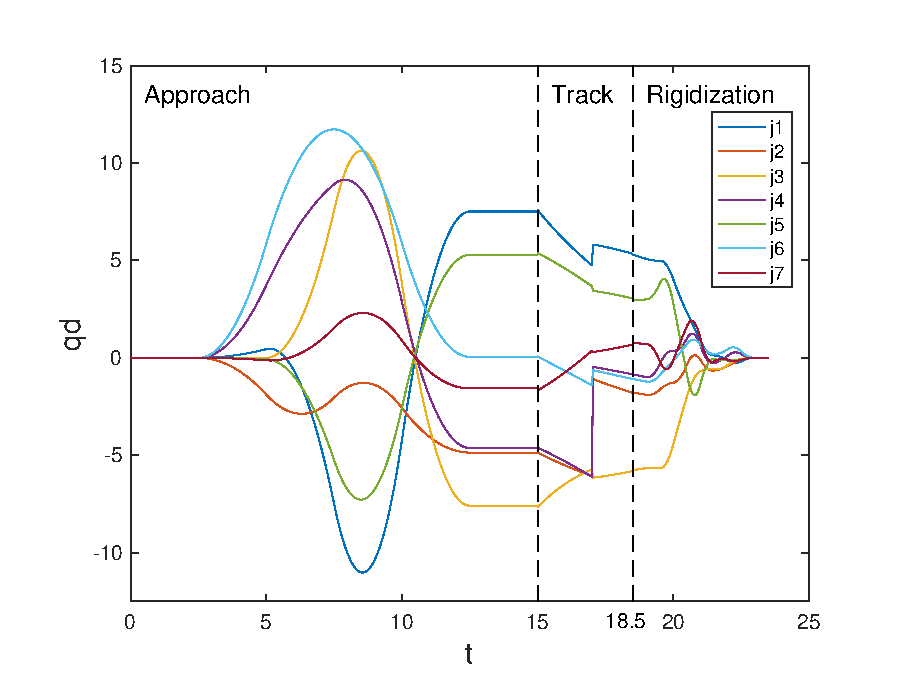
\includegraphics[angle=0,width=0.42\textwidth]{./figures/Joint_vel_2degs_2}
\caption{Simulated robot manipulator joint velocities for a Target spin velocity of 2 deg/s. The transition between the phases, at t=15~s and at t=18.5~s, is smooth. The jump during the tracking phase is due to the homing-in motion, which is however directed towards the target and, as such, does not have a noticeable effect on the pixel velocity in the camera image.}
\label{fig:Joint_vel_2degs}
%\vspace{-10pt}
\end{figure}
%
Fig.~\ref{fig:Joint_vel_2degs} shows the motion planner solution for a Target spin velocity of 2 deg/s. The figure shows the three phases of the maneuver. The transition from the approach to the tracking phase is smooth, as the end-effector alligns itself with the grasping point on the Target. The values of the parameters $\phi_{e \: mid}$ and $\phi_{e \: delta}$  were set to 40 and 7.5 deg respectively. The tracking phase lasts 3.5 seconds to allow for the gripper to close onto it. The rigidization phase \rev{starts after the Target is fully grappled and} lasts five seconds and the number of parameters per joint was $N_B=6$. The solution resulted from a global search,  which found different local minima, as expected, due to nonlinearity of the optimization problem. 

%The control gains were defined as ... $K_p$, $K_d$, nullspace K. The deadband filter of the Target force/torque sensor signals were set to 4N and 1Nm.

%
\begin{figure}[t!]
\psfrag{q}[cc][cc][\FontFigB]{$\MatO{q}-\MatO{q}{}_{ref}$ [deg]}
\psfrag{t}[cc][cc][\FontFigB]{$t$ [s]}
\centering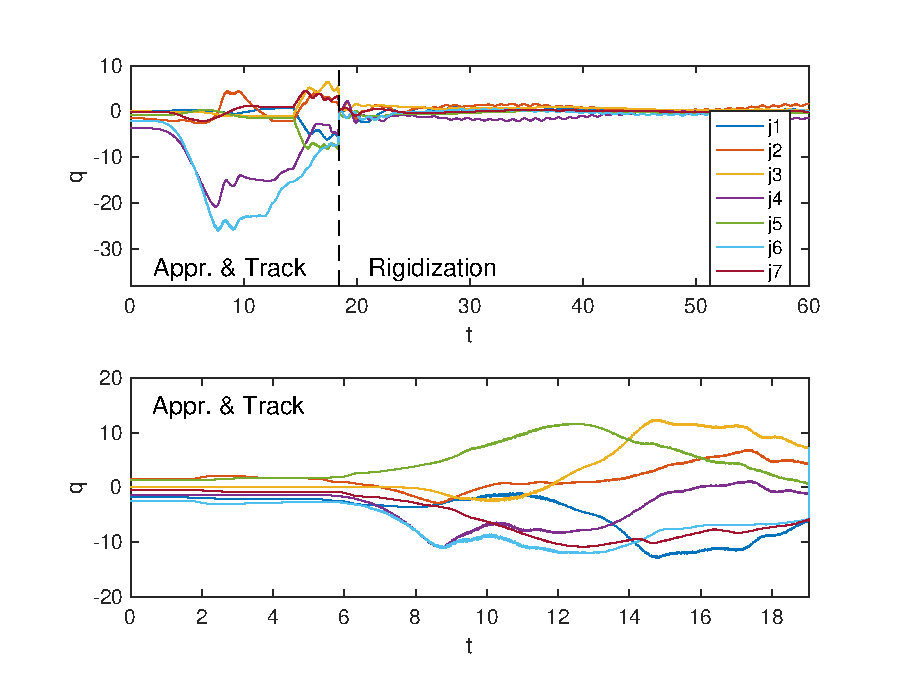
\includegraphics[angle=0,width=0.42\textwidth]{./figures/joint_space_motion_2subplots_2}
\caption{Measured robot manipulator joint position error for Target spin velocity of 1 deg/s (top) and 2 deg/s (bottom). For the latter case, only the approach phase is shown, in which however the use of the EKF and of the extended parameterization of the joint motion give a net increase in joint-space tracking performance.}
\label{fig:joint_space_motion_2subplots}
%\vspace{-10pt}
\end{figure}
%
%
\begin{figure}[t!]
\psfrag{xx}[cc][cc][\FontFigB]{$\MatO{\omega}{}_{t}$ [deg/s]}
\psfrag{yy}[cc][cc][\FontFigB]{$\MatO{\phi}{}_{t}$ [deg/s]}
\psfrag{t}[cc][cc][\FontFigB]{$t$ [s]}
\centering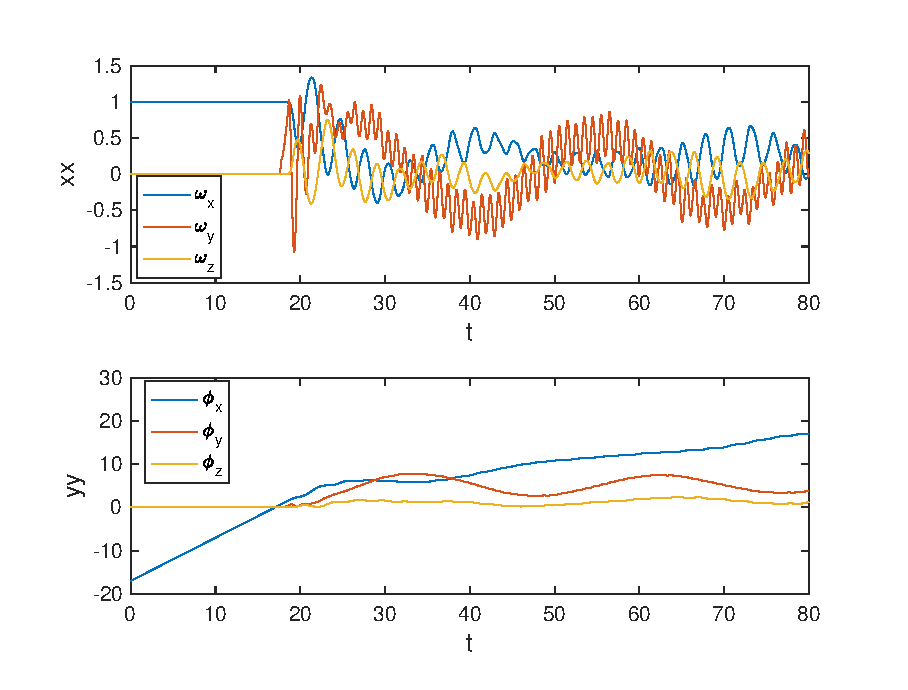
\includegraphics[angle=0,width=0.42\textwidth]{./figures/Target_motion}
\caption{Measured Target angular velocity (top) and orientation (bottom) for the 1 deg/s case. The post-grasping tumbling of the sattellite stack is visible in the (reduced) rotation about the $x$-axis.}
\label{fig:Target_motion}
%\vspace{-10pt}
\end{figure}
%

Fig.~\ref{fig:joint_space_motion_2subplots} shows the measured robot manipulator joint position error, defined as $\MatO{q}-\MatO{q}{}_{ref}$, for the cases of Target spin velocities of 1 deg/s and 2 deg/s respectively. In the experiments on the OOS-SIM facility it was in fact found that the rigidization task for the 2 deg/s case was intractable with the current setup. \rev{CHECK need motivation} As such the experimental results presented here for the rigidization phase only relate to the 1 deg/s case. In Fig.~\ref{fig:Target_motion} the measurement of the Target motion is shown, in which we observed a very slow damping of the angular velocity. \rev{The oscillations in the angular velocity appear to have two frequencies: the lower one is to be attributed to the imepdance control of the LWR; the higher one is to be attributed to the time delay and discretization effects in the control loop of the facility (independent of the LWR impedance parameters).}

%Furthermore, the inertial parameters of the two satellites used in the facility model were increased with respect to ideal values. This was done in order to limit the velocities commanded to the industrial robots. The values taken here were.... chaser, target inertias, L

Returning to Fig.~\ref{fig:joint_space_motion_2subplots}, the error in the joint position is shown to improve substantially for the second case, due to the fact that the EKF and the joint motion parameterization shown in Fig.~\ref{fig:Joint_vel_2degs} is used (the manuever was not possible without these new features). While the first provides a smoother estimate of $\MatO{H}{}_{ge}$ (as shown below), the latter reduces the pixel velocity by a factor of two. At the point of transition between the tracking and the rigidization phase ($t=18.5$), the joint position error becomes zero, due to the recomputation of the reference trajectory (see Section\ref{sec:rigidization}). The tracking error in the rigidization phase is then shown to remain small.

In Figures~\ref{fig:fig_norm_errors} the output error norm of the position $r_c$ of EKF and vision is compared with respect to the ground truth. The EKF error norm is plotted as a heat-map of the statistical metrix, $\chi^2$ of the incoming vision data. It is observed that the $\chi^2$ measure degrades (yellow) for $t > 0 $ and $||r_c|| \rightarrow 0 $. In Fig.~\ref{fig:fig_norm_errors}, the degradation of vision data culminates in measurement failures (marked as rectangular area) towards the end. The EKF estimates though stay bounded. Fig.~\ref{fig:states_EKF} shows the velocity convergence of the filter. It also demonstrates the orientation degradation as $||r_c|| \rightarrow 0$. This observation betrays a general problem with the eye-in-hand configuration of visual servoing, since, in close proximity to target, the observability degeneracy degrades camera-based measurement. 
%
\begin{figure}[t!]
\psfrag{y1}[cc][cc][\FontFigB]{$||\Delta r_c||^2$}
\psfrag{y2}[cc][cc][\FontFigB]{$||\Delta r_c||^2$}
\psfrag{leg1}[cc][cc][\FontFigM]{$EKF$}
\psfrag{leg2}[cc][cc][\FontFigM]{$Vision$}
\psfrag{x}[cc][cc][\FontFigM]{$EKF$}
\psfrag{y}[cc][cc][\FontFigM]{$Vision$}
\psfrag{t}[cc][cc][\FontFigB]{$t$[sec]}
\psfrag{ekf}[cc][cc][\FontFigM]{$EKF$}
\psfrag{vision}[cc][cc][\FontFigM]{$Vision$}
\centering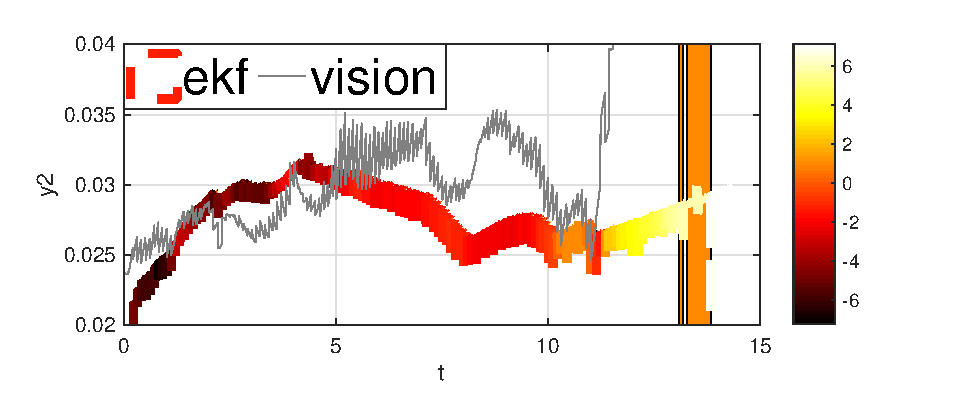
\includegraphics[angle=0,width=0.47\textwidth]{./figures/fig_norm_errors}
\caption{Comparison of direct-Vision measurements with EKF, based on the norm $||\Delta r_c^2||$. As $||r_c|| \rightarrow 0$, the statistical measure of fitness, $\chi^2 \rightarrow \infty $ eventually leading to pose estimation failures due to degenerate observability.}
\label{fig:fig_norm_errors}
%\vspace{-10pt}
\end{figure}
%
%
\begin{figure}[t!]
\psfrag{om}[cc][cc][\FontFigB]{$\omega$}
\psfrag{omhat}[cc][cc][\FontFigB]{$\hat{\omega}$}
\psfrag{true}[cc][cc][\FontFigB]{$\omega$}
\psfrag{t2}[cc][cc][\FontFigB]{$t$[sec]}
\psfrag{t1}[cc][cc][\FontFigB]{$t$[sec]}
\psfrag{qua}[cc][cc][\FontFigB]{$\mu$}
\psfrag{qhat}[cc][cc][\FontFigB]{$\hat{\mu}{}_{KF}$}
\psfrag{vision}[cc][cc][\FontFigB]{$\mu_V$}
\centering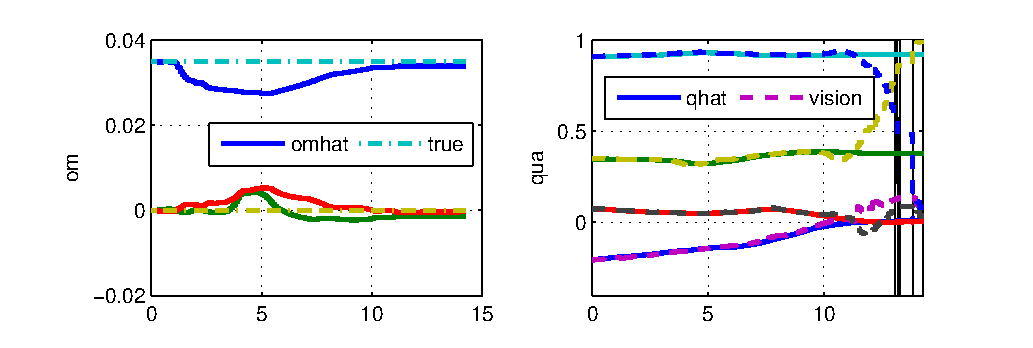
\includegraphics[angle=0,width=0.48\textwidth]{./figures/states_EKF}
\caption{a) Target state estimation ($\omega$) in EKF for tracking control. b) Divergence of visual tracking's orientation estimate towards end of maneuver.}
\label{fig:states_EKF}
%\vspace{-10pt}
\end{figure}
%
\section{Discussion and Conclusion}
\label{sec:disc}
%
The main achivement of this paper is to demonstrate the feasibility of a grasping strategy based on Target motion prediction, robot motion planning and trajectory tracking, specifically for the latter step. In fact, due to modelling uncertainties, the true trajectory deviates from the reference trajectory in joint space. The latter is therefore partially adapted online for the rigidizaiton phase. A method is presented and validated here, which does that while favouring joint position related motion constraints. The tracking controller is then shown to succesfully perform the task. In this way, the feasible (and optimal) motion planning solutions,  \rev{which describe trajectories for the full degrees of freedom of the system throughout the approach and rigidization phases, and which are} computed offline with much computational effort, are shown to be useful for control purposes. %The reference trajectories are computed taking a complete three-dimensional multibody dynamics model into consideration, without simplifying assumptions.
%
%We also argue that a reference trajectory based method provides greater robustness than local control methods. The control method must provide a guarantee that the grasping point can be tracked at all times and that the rigidization phase which follows remains feasible. Local control (e.g., potential) methods generally cannot provide this guarantee. Free-floating robots are known to possess dynamic singularities, which are function of the related distribution of its inertia. Their position in joint space, for the multibody system of interest here, is not only to the author's knowledge not representable, but is also variable in time during the robot's operations, due to changes in the inertial distribution. 

A second major achievement of this paper is the implementation of an Extended Kalman Filter \rev{in between the visual tracker and the visual servo in cascade with an impedance controller. This} ensures a Lipschitz continuity of measurements during the robot motion CHECK (make clear why this is not a trivial engineering step), making the control method robust for executing the grasping task. It is in fact shown that the visual tracking algorithm adoped may become degenerate in the vicinity of the Target (CHECK but Aghili does this too). Furthermore, the new formulation to reduce the computational footprint has been shown to give a signifcant improvement (CHECK where?). %Finally, given that the visual servo along with manipulator dynamics is known to lose passivity in presence of target motion [], the computation of the reference trajectory provides the necessary feedforward terms which ensure passivity unter the assumption of no modelling errors. This is complemented by the estimate of the Target velocity provided by the Kalman filter, as shown in Fig.\ref{fig:states_EKF}. As a result, the overall system is passive in the absence of external torques on the Target.

%A limitation of the presented method is however also recognized. We argued, in fact, that the modelling uncertainties are small and as such, by grossly tracking the reference trajectory, the feasibility of the complete maneuver is guaranteed. In reality, the reference trajectory is only feasible at predefined via points along it, given the time discretization of the optimal control problem. This does not say anything about the feasibility of the solution in its vicinity. Future work will need to address this robustness issue, given that the tracking controller departs from the reference trajectory to account for the uncertainties. 

The momentum-based approach on the OOS-SIM facility has proven to be efficient in reducing drift due to noise and modelling errors. Future work will be dedicated to improving its performance in the coupled configuration. Furthermore, the stability of complete interconnected system will be addressed. Finally, the sensing of the Chaser, to include typical sensor noise and sampling times, will be considered.
%
%
%"In this way, by grossly tracking the reference trajectory the feasibility of the complete maneuver is guaranteed. As such, the end time of the stabilization phase need not be minimal, as suggested in [Aghili], since it is sufficient that the system remains in the vicinity of the planned trajectory, and may be chosen following a different cryterion. Minimum energy maneuvers can be considered as a viable alternative, since, as we will see, they are more robust to modelling errors and visual servo inaccuracies."
%
%Following target trajectory and slowing it down does not take account of chaser inertia. Providing a MBS solution vs Aghili's single rigid body solution.
%
%The satellite states are assumed to be ideal
%
%
%\section{Videos}
%1. simulation - bernhard
%2. facility
%@unknown{unknown,
%author = {Isabel Ribeiro, Maria and Ribeiro, Isabel},
%year = {2004},
%month = {04},
%pages = {},
%title = {Kalman and Extended Kalman Filters: Concept, Derivation and Properties}
%}


%%%%%%%%%%%%%%%%%%%%%%%%%%%%%%%%%%%%%%%%%%%%%%%%%%%%%%%%%%%%%%%%%%%%%%%%%%%%%%%%

%\section*{ACKNOWLEDGMENT}

%The preferred spelling of the word �acknowledgment� in America is without an �e� after the �g�. Avoid the stilted expression, �One of us (R. B. G.) thanks . . .�  Instead, try �R. B. G. thanks�. Put sponsor acknowledgments in the unnumbered footnote on the first page.



%%%%%%%%%%%%%%%%%%%%%%%%%%%%%%%%%%%%%%%%%%%%%%%%%%%%%%%%%%%%%%%%%%%%%%%%%%%%%%%%

%References are important to the reader; therefore, each citation must be complete and correct. If at all possible, references should be commonly available publications.

\bibliographystyle{ieeetr} % this style is typical of the ieee, but there are others!
\bibliography{Biblio} % run 'bibtex root' befire running 'latex root'!


\end{document}
